\section{Data Preparation}

Before introducing the datasets we use, we first need to learn some tools to use on those datasets. We use the Fourier transform and normalization for data preparation.

\subsection{Fourier Transform}

Fourier transform on $\mathbb{R}$ is a mathematical operation that transforms the input into the frequencies. The frequency function by Fourier transform gives a complex-valued function on $\mathbb{C}$. There are two Fourier transform types: Continuous Fourier Transform (CFT) and Discrete Fourier Transform (DFT or DtFT)~\cite{four}.

\subsubsection{CFT}

As we can understand from the name, the Continuous Fourier Transform uses a continuous function, $x(t)$, as a time signal function with frequency function $f$ to transform into frequency representation, $X(f)$. There are two versions of CFT, where one is Direct in Equation~\eqref{direct}, and the other one is Inverse in Equation~\eqref{inverse}~\cite{four}. The inverse Fourier transform allows us to return to the original signal from frequency transformation. If we take $i = \sqrt{-1}$ (imaginary unit), then:
\vspace{10pt}

\begin{subequations}
\label{fourier calc}
\renewcommand{\theequation}{\theparentequation.\arabic{equation}}
    \noindent\text{Direct:}
    \begin{equation}
   X_{\text{CFT}}(f) = \int_{- \infty}^{\infty} x(t)\cdot e^{-i2\pi ft}dt\label{direct}
    \end{equation}
    \text{Inverse:}
   \begin{equation}
    x_{\text{CFT}} (t) = \int_{- \infty}^{\infty} X(f)\cdot e^{i2\pi ft}df\label{inverse}
   \end{equation}
    \end{subequations}
\vspace{10pt}

Since our transform function has $e^{i}$, is the complex value we can dissect the exponent to $\cos$ and $i\sin$ values for simplicity as Equation~\eqref{expo}, and rewrite the Fourier equation like in Equation~\eqref{simpf}.
\vspace{10pt}

Since;
\begin{equation}
  e^{i\theta} = cos(\theta) + isin(\theta), \quad\forall \theta \in [0,2\pi)
  \label{expo}
\end{equation}
\vspace{10pt}

Then;
\begin{equation}
\begin{split}
  X_{\text{CFT}} (f) &= \int_{-\infty}^{\infty} x(t)\cdot e^{-i2\pi ft}dt \\
  \\
 &=\int_{-\infty}^{\infty} x(t)\cdot \cos(2\pi ft)dt - i\int_{-\infty}^{\infty} x(t)\cdot \sin(2\pi ft)dt \label{simpf}
\end{split}
\end{equation}


\subsubsection{DFT}

DFT is the discrete counterpart of CFT and is used when we have discrete valued inputs (discrete-time signals). We are interested in DFT since the inputs we use for the LVQ model in this paper are discrete values. In DFT, we take $x(n)$ for time signals instead of $x(t)$ to indicate discreteness, where $n \in \mathbb{N}$. Then, the DFT formula will be:
\vspace{10pt}

\begin{equation}
\begin{split}
  &X_{\text{CFT}}(f) = \int_{-\infty}^{\infty} x(t)\cdot e^{-i2\pi ft}dt \\
  \\
  \implies& X_{\text{DFT}}(f) = \sum_{n = -\infty}^{\infty} x(n\cdot \Delta t)\cdot e^{-i2\pi f(n\cdot \Delta t)}\label{dft}
\end{split}
\end{equation}
\vspace{10pt}

As we can see from the Equation~\eqref{dft}, DFT has a similar calculation to CFT. The difference is that instead of using integral, we are using infinite sums because of the discreteness of DFT. Since the domain is discrete, we need to arrange the summation step accordingly. If $f_{s}$ is the sampling frequency, we can denote the period as $\Delta t = \frac{1}{f_{s}}$. Then, the time $t$ would be $ t = n \cdot \Delta t $. We can further transform the Equation~\eqref{dft} into the Equation~\eqref{dftdir} and find the inverse of DFT equation as in the Equation~\eqref{dftinv}~\cite{four}:
\vspace{10pt}

\begin{subequations}
\renewcommand{\theequation}{\theparentequation.\arabic{equation}}
\noindent Direct (Analysis):
\begin{equation}
X_{\text{DFT}} (\frac{f}{f_{s}}) = \sum_{n = -\infty}^{\infty}x(n)\cdot e^{-i2\pi \frac{f}{f_{s}}n}\label{dftdir}
\end{equation}
Inverse (Synthesis):
\begin{equation}
x_{\text{DFT}} (n) = \frac{1}{f_{s}}\int_{-fs/2}^{fs/2}X(\frac{f}{f_{s}})\cdot  e^{i2\pi \frac{f}{f_{s}}n}df\label{dftinv}
\end{equation}
\end{subequations}
\vspace{10pt}

Since $e^{i2\pi \frac{f}{f_{s}}n}$ is periodic, we do not need to calculate the equation for both $n>0$ and $n<0$ to save time and calculation power~\cite{four}. Then, we can get the final equation, Equation~\eqref{simpdft} for DFT with finite signals $|S| = N$~\cite{four}.
\vspace{10pt}


\begin{equation}
X_{\text{DFT}} (\frac{f}{f_{s}}) = \frac{1}{N}\sum_{n=0}^{N-1}x(n)\cdot e^{-i2\pi \frac{f}{f_{s}}n}, \quad -f_{s}/2 \leqslant f < f_{s}/2\label{simpdft}
\end{equation}
\vspace{10pt}



We do not directly transform the math into code but use a Python library, NumPy, to use the Fourier transform. The function is the Fast Fourier transform, and it uses DFT.
\vspace{10pt}

\noindent More on NumPy’s Fourier transform at:

\noindent \url{https://numpy.org/doc/stable/reference/generated/numpy.fft.fft.html}

\subsection{Normalization}

Normalization is a statistical process to reduce the feature ranges to the same scale. It is essential to use normalization in some datasets since some features in datasets might have bigger range differences than others, and this difference shifts decision-making to the bigger range in machine learning methods. The weight vector can adjust the range difference in weight vector-based machine learning models. However, in prototype-based models, we do not have many options.

We use squared Euclidian distance in LVQ models, and the closeness to the given sample selects the winner. Suppose one of the features has a greater range difference than other features. In that case, that feature contributes the overall distance more than other features, resulting in the model’s decision on the given sample being based mostly on that feature.

There are several normalization methods, and the common ones are min-max scaling (scaling to a range), clipping, log scaling, and z-score ~\cite{googledev}. We use scaling to a range method in our paper, so we talk about it. If someone is curious about other methods, please visit the link by \href{https://developers.google.com/machine-learning/data-prep/transform/normalization}{developers.google} or source~\cite{googledev} to learn more.

\subsubsection{Min-max scaling}
The scaling method scales the features in the range $[0,1]$. The method transforms the feature $x_{i}$ of array $\mathbb{x}$ into $\hat{x}_{i}$ by:
\vspace{10pt}


\begin{equation}
\hat{x}_{i}= \frac{x_{i} - min(X_{i})}{max(X_{i}) - min(X_{i})}\label{norm}
\end{equation}
\vspace{10pt}

Here in the Equation~\eqref{norm}, $min(X_{i})$ and $max(X_{i})$ represent the minimum an maximum values of the i$^{th}$ element between all the feature arrays in a given dataset X, respectively.

\section{Creating Datasets from IFE Data}\label{creIFE}

\subsection{What is un/structured data?}

First, we need to understand what structured and unstructured data is. Structured data is the data that we can store in spreadsheets. These data have column names and rows for each data. Structured data columns can be strings, numerical, datetime, Boolean, or null values. Anything other than structured data, we call all data unstructured data. This data type contains image data, video data (which is also a type of image data with order), audio data, and text data. We would be using image data to train our algorithms, so we talk about how we use the image data to train machine learning algorithms and skip the other unstructured data types. We mentioned that machine learning algorithms require numerical values, but an image is hard to imagine as a numerical value. The idea of using images as data for machine learning is to use pixel values of the data. Of course, we can use raw pixel values to train the algorithm, but to increase performance, we can convolute the pixel values for different algorithms. The machine learning methods in this paper use structured data, so we will not go deep into the concept and how to use unstructured data for machine learning.

\subsection{Cross-correlation}

We use (discrete) cross-correlation to detect the bars in our data. That is why, first, we need to understand what cross-correlation is. Since our data contain 2-dimensional images, we talk about 2-dimensional cross-correlation on images. Cross-correlation is similar to convolution, and the only difference is that in convolution, we rotate the second component (kernel) and then do the cross-correlation operation. If the kernel values are uniform, then the output of cross-correlation and convolution would give the same result. (Discrete) cross-correlation in Equation~\eqref{cros} and (Discrete) convolution in Equation~\eqref{conv}.
\vspace{10pt}


    \begin{equation}
x(n) \ast y(n) = \sum_{k=0}^{\infty}y(k)\cdot x(n+k)\label{cros}
    \end{equation}

    \begin{equation}
x(n) \otimes y(n) = \sum_{k=0}^{\infty}y(k)\cdot x(n-k)\label{conv}
    \end{equation}
\vspace{10pt}


There are many ways to use cross-correlation in mathematics and computer science. Cross-correlation and convolution are used mostly with images to extract information from the image. Cross-correlation starts with a kernel (in a 2-dimensional case, we can see a kernel as a 2-dimensional array or a matrix). The kernel values run over all the image data. For every step, the kernel does an elementwise multiplication with the rows and columns of the matrix to create a combined value for the given position regarding kernel values. For example, if the kernel size is a $3 \times 3$ matrix with $\frac{1}{9}$ for each of the kernel values, then the kernel takes the mean of the image values with radius 1 pixel. So, using the cross-correlation (or convolution) operation makes our image more compact or blurry depending on the kernel’s step size (stride). The kernel values can get any value, and different kernel values can find different aspects of the data that cross-correlation works on. We saw how to blur the image by taking the mean of surrounding pixel values. However, if we pick the top row of the $3 \times 3$ cross-correlation kernel as $+\frac{1}{3}$ and the bottom row as $-\frac{1}{3}$, the kernel finds the horizontal lines in the given image data.

After deciding the kernel size and values, we must also decide the kernel’s step size. As we mentioned, step size also changes the interpretation of the convoluted image. If we take a $3 \times 3$ kernel and $\text{step size} = 3$, the image will shrink to one-third. However, if we take step size to 1 for the same example, we achieve a blurred image with the same size as the original image.

Lastly, we have a padding option for the cross-correlation and convolution. The padding adds empty spaces to our image’s border. We add padding to adjust the image shape to our liking. Without any padding, the edge of the image will always be convoluted with the edge value of the kernel, but if we add padding, we give the edge values of the image a better chance to be in the center of the kernel.

We do not need a rectangular kernel or padding or stride to the width and height of the image. We can choose different sizes for stride and padding to width and height values. After passing through one convolution operation, the new image size changes for height and width given in Equation~\eqref{convh} and ~\eqref{convw}, respectively.

\begin{itemize}
\item $\text{H}_{\text{in}} = \text{input height}$

\item $\text{W}_{\text{in}} = \text{input width}$

\item $\text{H}_{\text{out}} = \text{output height}$

\item $\text{W}_{\text{out}} = \text{output width}$
\end{itemize}

\begin{subequations}
\label{convhw}
\renewcommand{\theequation}{\theparentequation.\arabic{equation}}
    \begin{equation}
    \text{H}_{\text{out}} = \lfloor \frac{\text{H}_{\text{in}} + 2 \times \text{H}_{\text{padding}} - \text{H}_{\text{dilation}} \times (\text{H}_{\text{kernel size}} - 1) -1}{\text{H}_{\text{stride}}} +1 \rfloor \label{convh}
   \end{equation}
   \vspace{5pt}
   \begin{equation}
   \text{W}_{\text{out}} = \lfloor \frac{\text{W}_{\text{in}} + 2 \times \text{W}_{\text{padding}} - \text{W}_{\text{dilation}} \times (\text{W}_{\text{kernel size}} - 1) -1}{\text{W}_{\text{stride}}} +1 \rfloor \label{convw}
   \end{equation}
\end{subequations}
\vspace{10pt}

\noindent The equations in ~\eqref{convhw} are adapted from PyTorch documentation.
\vspace{10pt}

\noindent For more information:

\noindent \url{https://pytorch.org/docs/stable/generated/torch.nn.Conv2d.html#torch.nn.Conv2d}

\subsection{Where is our data coming from?}

We use IFE (immunofixation electrophoresis) test results to create datasets for our models to test. Our data is image data and contains 6 bars. We will not use the image as the input for our machine learning methods; instead, we will transform the image data into structured data to train the OGLVQ and CGLVQ methods.

IFE samples can be either blood or urine samples, but the IFE data uses blood samples~\cite{mypap}. The test can help to diagnose various diseases. The IFE test can detect problems such as~\cite{testing}:

\begin{itemize}
    \item Help in the diagnose and monitoring of lymphoma, chronic lymphocytic leukemia, or monoclonal gammopathies, such as multiple myeloma
    \item Investigate abnormal findings on other laboratory tests, such as total protein, albumin level, elevated calcium levels, or low white or red blood cell counts
    \item Evaluate someone for an inflammatory condition, an autoimmune disease, an infection, a kidney or liver disorder
\end{itemize}
Note: Adapted from Testing.com. (2021, March 24). Protein Electrophoresis, Immunofixation
Electrophoresis, Testing.com \url{https://www.testing.com/tests/protein-electrophoresis-immunofixation-electrophoresis/}~\cite{testing}.
\vspace{10pt}

The IFE test is used to detect the abnormal globulin values in the sample. Immunoglobulins are proteins in the blood that contain a pair of heavy and light chains. $\alpha$ (Alpha), $\gamma$ (Gamma), and $\mu$ (Mu) are the heavy chains, and these heavy chains combine with one of the light chains; $\kappa$ (Kappa) or $\lambda$ (Lambda), to form immunoglobulin as seen on the Figure~\ref{globulin}.

\begin{figure}[H]
\centering
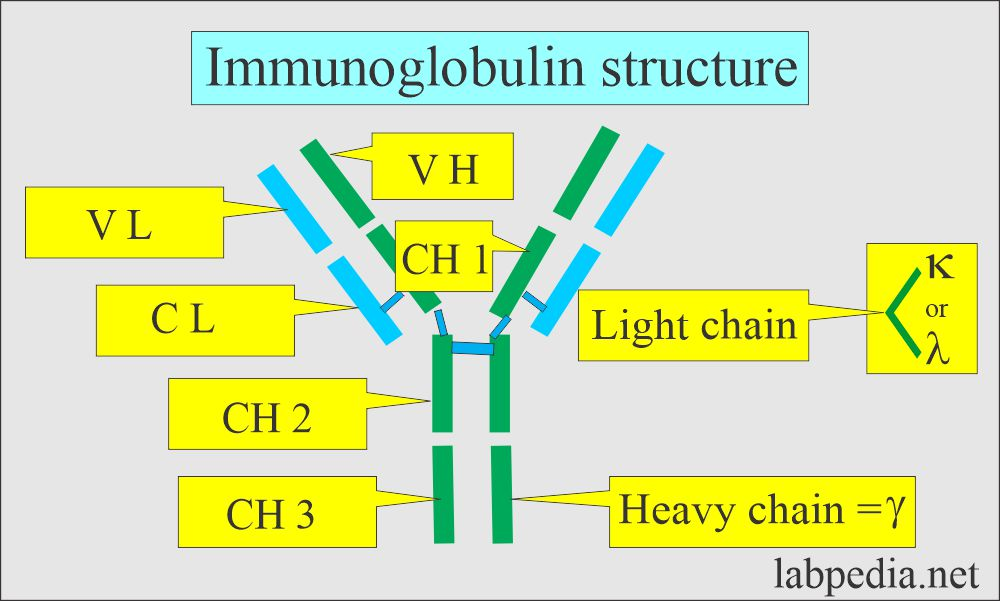
\includegraphics[width=.99\textwidth]{images/old imgs/Immunoglobulin-structure.jpg}
\caption{Immunoglobulin structure.}
\label{globulin}
\end{figure}

\noindent Note: From "Monoclonal Immunoglobulin (Ig), Monoclonal antibody, Immunofixation Electrophoresis (IFE)" by Labpedia.net. (2020, January 25) \noindent\url{https://labpedia.net/monoclonal-immunoglobulin-ig-monoclonal-antibody-immunofixation-electrophoresis-ife/}~\cite{labpediaa}.
\vspace{10pt}

IFE test samples have 6 bars: $SP$ (Serum Protein Electrophoresis) bar or Marker bar, $\gamma$ bar, $\alpha$ bar, $\mu$ bar, $\kappa$ bar, and $\lambda$ bar from left to right can also be seen in Figure~\ref{IFE}. In Figure~\ref{SP}, we see the $SP$ bar contains 6 bands, namely; albumin, $\alpha-1$ (Alpha-1), $\alpha-2$ (Alpha-2), $\beta-1$ (Beta-1), $\beta-2$ (Beta-2), $\mu$ (Mu), and $\gamma$ (Gamma) from top to bottom. The $SP$ bar quantitively measures the albumin and globulins in the blood sample, so we cannot compare which globulin is abundant in the sample by just looking at the $SP$ bar~\cite{leung}. However, just checking the $SP$ bar, we can detect if any of the globulin in the sample is abnormal, which would be useful to distinguish healthy and unhealthy patients. Except for the $SP$ bar, the rest of the bars in IFE results measure the globulins qualitatively, so we can compare the bars and find which globulins are abundant in the blood sample.

\begin{figure}[H]
\centering

\begin{subfigure}[t]{0.50\textwidth}
\centering
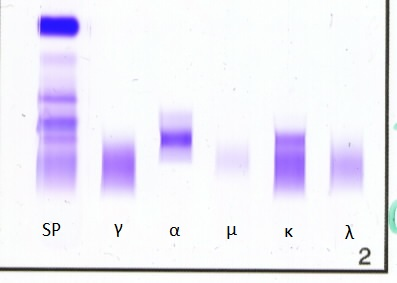
\includegraphics[width=1\textwidth]{images/old imgs/IFE_names.jpg}
\caption{Sample IFE image.}
\label{IFE}
\end{subfigure}
\hfill
\begin{subfigure}[t]{0.40\textwidth}
\centering
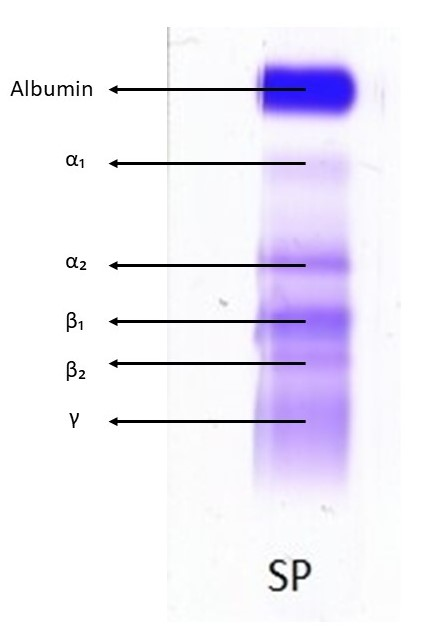
\includegraphics[width=1\textwidth]{images/old imgs/sp_name.jpg}
\caption{Sample image's SP part. These band name positions are just representative to show the order of the band names, and should not be taken as exact correct places for the bands.}
\label{SP}
\end{subfigure}

\caption{IFE and SP images.}
\end{figure}

\noindent Note: Adapted from "Informational Image Data Preprocessing: IFE Blood Samples
[Unpublished manuscript]" by M. Saruhan, Applied Mathematics for Network and Data Sciences,
Mittweida University of Applied Sciences, p. 2 ~\cite{mypap}.
\vspace{10pt}

When an immunoglobulin is more abundant than it should be, we name the case the abundant immunoglobulin’s name. For example, if the sample is marked as IgM-$\lambda$, the test found immunoglobulin $\mu$-$\lambda$ more than it should be in the sample. We have eight different diagnoses in our dataset, of which 6 of the types are labeled as unhealthy results with abundant immunoglobulin: IgA-$\kappa$, IgA-$\lambda$, IgM-$\kappa$, IgM-$\lambda$, IgG-$\kappa$, IgG-$\lambda$ in their blood, one is healthy and the last one is unclear diagnosis.

We mentioned alpha and gamma for bands in the $SP$ bar and bars in the IFE test results. While $\alpha$ and $\gamma$ in IFE results represent the globulins, they do not represent the same in the $SP$ bar. In the $SP$ bar, $\alpha$ and $\gamma$ are just band names. The similar name usage might be confusing, so read carefully that we talk about $\alpha$ bands in the $SP$ bar or $\alpha$ globulin in IFE results.

The machine that gives the immunofixation results groups the albumin and globulin by their electrical charge~\cite{eclinpath}. The grouping can be mostly visible in the $SP$ bar since the bar has albumin and different globulins altogether in the sample. Albumin is the most abundant in the blood sample and has the most negative charge than globulins~\cite{leung}. Because of this reason, albumin has a distinct thickness and position in the $SP$ bar.

\subsection{Transforming to structured data}

We need to pre-process the bar image data into structured data to prepare it for use in GLVQ models. We use the pre-processing of bar image data according to the report from Saruhan (2023), and the pre-processing we use in this paper is taken from that report~\cite{mypap} until we transform the data into a dataset. According to the report~\cite{mypap}, we need one reference image for creating an albumin mask to find the $SP$ bar position on each image file, another reference image for approximating the length of the bars, and one last reference image for finding the approximate distance between each bar.

After extracting the albumin mask from the respective reference image, we create a kernel (matrix) that is the same size as the albumin mask and has values one everywhere. We use this kernel to calculate the cross-correlation with the images to find the albumin’s position in every image in our data. The kernel runs over any image and finds the position where it gets its maximum value. Since the albumin on each image file has a high pixel value, we expect to get the maximum value at the exact place of the albumin. However, to find the position of the albumin, we use a kernel with value one, and we do not need to convolute the kernel across the whole image. We know the albumin is located on the top-left part of each image, so checking the maximum value of the cross-correlation at the top-left part would be enough. An example of how the search with the albumin mask works can be seen in Figure~\ref{findalbumin}.

\begin{figure}[H]
    \centering
    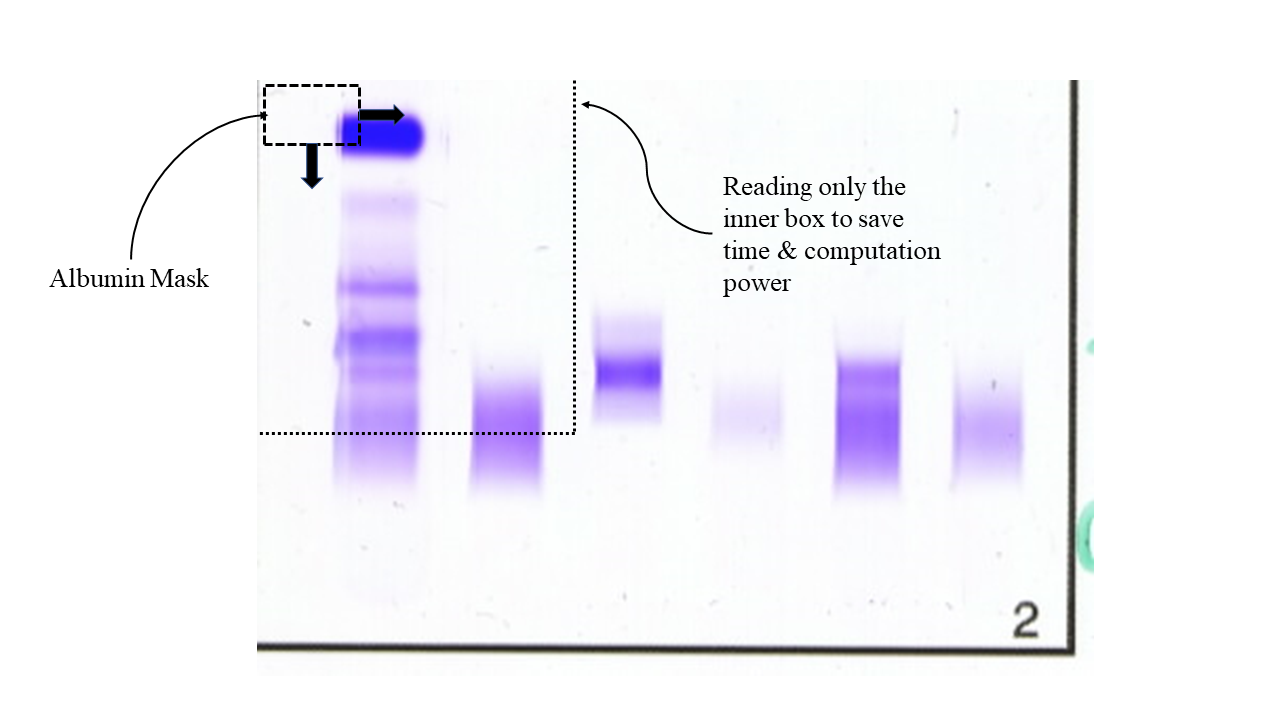
\includegraphics[width=0.98\textwidth]{images/old imgs/mask_in_use.png}
    \caption{Finding mask's maximum value to detect albumin on test image.}
    \label{findalbumin}
\end{figure}

\noindent Note: Adapted from "Informational Image Data Preprocessing: IFE Blood Samples
[Unpublished manuscript]" by M. Saruhan, Applied Mathematics for Network and Data Sciences,
Mittweida University of Applied Sciences, p. 2 ~\cite{mypap}
\vspace{10pt}

Since we now can locate the $SP$ bar, we can use it on our second reference image, approximating the length of the bars. After finding the $SP$ bar in our second image, we find the length of the bar by checking the values of the $SP$ bar from bottom to top. We find the position where the pixel values at the $SP$ bar position pass a given threshold and mark the transaction position as the bottom of the $SP$ bar. We can see the example of how to find the bottom line of the bar in Figure~\ref{bot2top}. Since we already found the top of the albumin with the albumin mask, we take the top of the albumin, the same as the top of the $SP$ bar, and calculate the difference from the bottom line we found. The difference would be the length of the SP bar.

\begin{figure}[H]
    \centering
    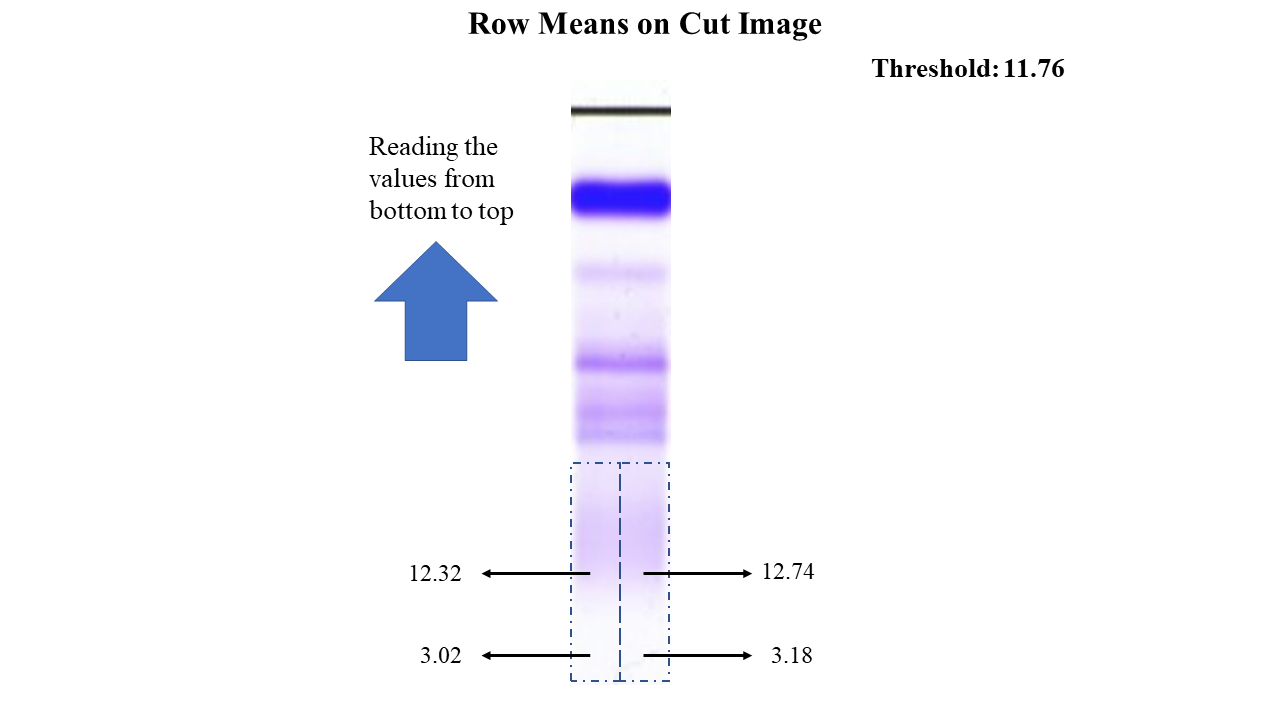
\includegraphics[width=0.98\textwidth]{images/old imgs/lenght_detection.png}
    \caption{Finding bottom index of the bar.}
\label{bot2top}
\end{figure}

\noindent Note: Adapted from "Informational Image Data Preprocessing: IFE Blood Samples
[Unpublished manuscript]" by M. Saruhan, Applied Mathematics for Network and Data Sciences,
Mittweida University of Applied Sciences, p. 2 ~\cite{mypap}
\vspace{10pt}

After finding the $SP$ bars’ position and length in every image, we need to find the other bars. To find other bars, we use our third reference image. We use reference images because every bar pair distance is nearly the same in every image. So, we can find the distances from one image and implement them to others, which saves us lots of computational power and time. In this image, we first use an albumin mask to locate the $SP$ bar to find our starting point. After finding the $SP$ bar, we create a bar mask using the dimensions of the $SP$ bar we found using albumin and length reference images. Same process as $SP$ location using albumin mask, we use $SP$ bar mask to locate other bars. The $SP$ bar mask also has values one everywhere. Since every bar is ordered next to each other, we do not want to go all the way in the bar row and calculate the cross-correlation of the mask and the image. If we do that, we locate the bar with the maximum value with the kernel, which might not be the next bar after the SP bar. So, we need to take cross-correlation until the end of the next bar. Figure~\ref{bar_detect} shows how the method finds the second bar, $\gamma$ bar. After finding the second bar, we can use the same process on the second bar to find the third bar, and so on. Lastly, to find the distances between each bar, we can use the distance information on other images to find the other bars after finding the SP bar via an albumin mask.

\begin{figure}[H]
    \centering
    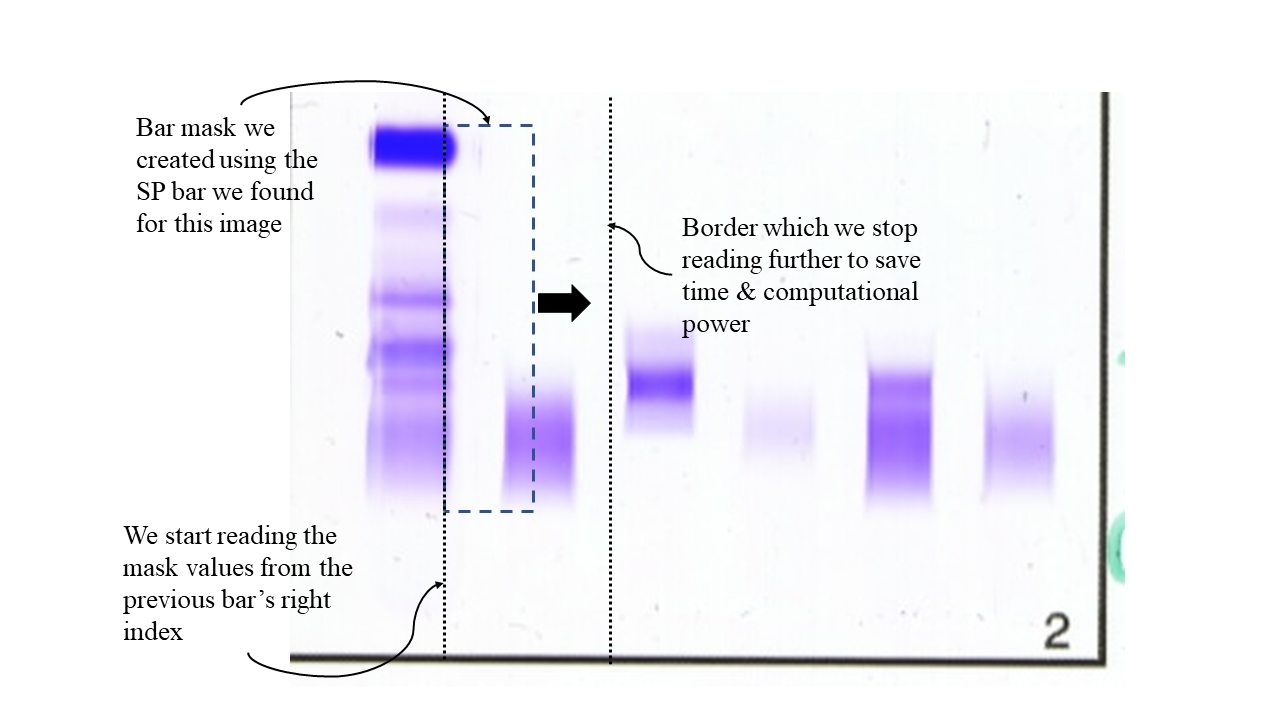
\includegraphics[width=0.98\textwidth]{images/old imgs/bar_detect.png}
    \caption{Example: Using detected SP bar as a mask to find other bars.}
    \label{bar_detect}
\end{figure}

\noindent Note: Adapted from "Informational Image Data Preprocessing: IFE Blood Samples
[Unpublished manuscript]" by M. Saruhan, Applied Mathematics for Network and Data Sciences,
Mittweida University of Applied Sciences, p. 2 ~\cite{mypap}.
\vspace{10pt}

Now, we have all the bar locations in all the images, so it is time to extract the bar values to structure and organize data. We extract the bar values in the image’s grayscale since we want to take the mean values for each row. As we mentioned, the positions of the bars are approximate. To get the correct value of the bars with confidence, we take the mean values of each row of the bar from the center of the bar with some small radius. This process helps us not to count the border of the bars since borders contain the background value of the images and could give us the wrong measure if we include the borders.

After reading each of the bar values for all our images, we get six arrays: $SP$, $\gamma$, $\alpha$, $\mu$, $\kappa$, and $\lambda$. The bar images and the corresponding value graphs are given in Figure~\ref{graphs}. We have bar values to use as input for our models, but another way to use bars as input is to use the frequency of each bar. IFE bars (especially SP bars) have density changes in color. Since we have bars with color grading, to find the density of the bar values, we transform the bar values into the frequency of the values with the help of the Fourier transform. The Fourier transform is taken here because the bars’ pixel values might differ for similar samples. Some samples might have tinted than others. However, if we look at the Fourier transform (DFT in this case) of each bar, we would be looking at the frequency of the bar, which differentiates the sudden changes on the bar better than without using the Fourier transform. We use DFT on all the bars separately on IFE blood test data because we do not want any relation between the end of each bar and the top of the next bar.

\begin{figure}[H]
    \centering
\begin{subfigure}[!t]{0.8\textwidth}
\centering
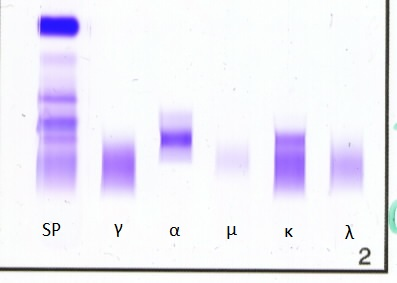
\includegraphics[width=1\textwidth]{images/old imgs/IFE_names.jpg}
\caption{Test IFE image.}

\end{subfigure}
\begin{subfigure}[!b]{0.90\textwidth}
\centering
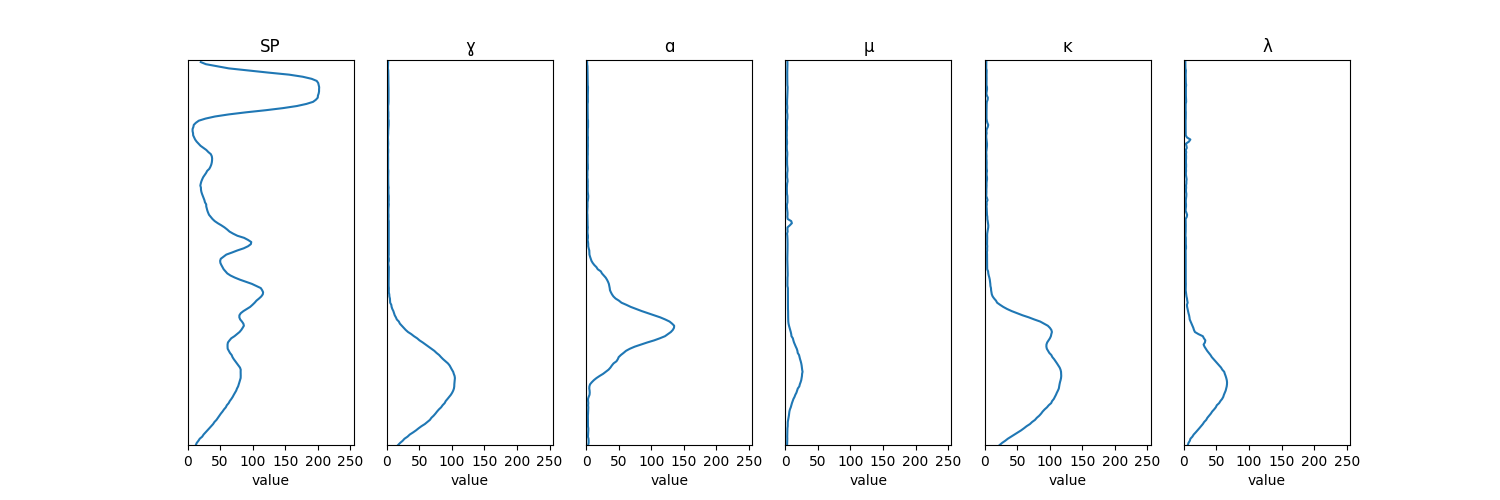
\includegraphics[width=1\textwidth]{images/old imgs/graph.png}
\caption{Graphs, created by reading the grayscale test image's bars.}

\end{subfigure}
    \caption{Extracting the image values into structured data.}
    \label{graphs}
\end{figure}

\noindent Note: Adapted from "Informational Image Data Preprocessing: IFE Blood Samples
[Unpublished manuscript]" by M. Saruhan, Applied Mathematics for Network and Data Sciences,
Mittweida University of Applied Sciences, p. 2 ~\cite{mypap}.
\vspace{10pt}

After we take each bar’s Fourier transform separately, we combine the results in one 1-dimensional array since to use the bar values in a machine learning method as input, we need to flatten the bar values into a 1-dimensional array.

According to Leung (2016), the $SP$ bar is used quantitively, showing if the patient is sick or not but not what kind of sickness~\cite{leung}. The $SP$ bar is useful for distinguishing sick patients, so we should include it in our dataset. However, the sickness is also shown in the other bars, and the $SP$ bar and the $SP$ bar have broader values than others, which results in models taking the $SP$ bar into account more than the other bars. So, to test both approaches, we create two datasets: one with the $SP$ bar included and one without the $SP$ bar. We name the dataset that the $SP$ bar included as \textit{SP} and the dataset that does not have the $SP$ bar as a feature named as \textit{NSP} (noSP).

We also have labels for the images which are given to us. The labels contain “IgA-$\kappa$” (Ak), “IgA-$\lambda$” (Al), “IgM-$\kappa$” (Mk), “IgM-$\lambda$” (Ml), “IgG-$\kappa$” (Gk), “IgG-$\lambda$” (Gl), “without any sickness” (wo), and “unclear decision” (ud). “Unclear decision” cannot be used with the other labels since it does not give us a clear answer. We store the remaining labels next to the bar values for each image data we transform.

At the end, we have two values in each row for both of the datasets; one is the input, which is the combination of the bar values we read, and the second one is the label of the data, which has seven different class discluding unclear decision as a label.

\section{Datasets}

Let us start by introducing the datasets we use in this paper. The datasets \textit{Glass}, \textit{Ionosphere}, \textit{Iris}, and \textit{Sonar} datasets we use, used in the results of the report “Self-incremental learning vector quantization with human cognitive biases”~\cite{lrimp}. Additionally, we added the \textit{Breast Cancer Wisconsin} Dataset~\cite{cancer} to our experiments to increase the variety. Since the features have distinct range differences, we use normalization on the \textit{Breast Cancer Wisconsin} and \textit{Iris} Dataset.

\subsection{Breast Cancer Wisconsin dataset}

The \textit{Breast Cancer Wisconsin} dataset was collected and computed from a digitized image of a fine needle aspirate (FNA) of a breast mass~\cite{cancer}. Dataset has two classes: Diagnosis “Malignant” (M) and “Benign” (B), which are the diagnoses given to the patient. The dataset contains ten central values:

\begin{itemize}
\item radius (mean of distances from the center to points on the perimeter)
\item texture (standard deviation of gray-scale values)
\item perimeter
\item area
\item smoothness (local variation in radius lengths)
\item compactness (perimeter$^{2}$ / area - 1.0)
\item concavity (severity of concave portions of the contour)
\item concave points (number of concave portions of the contour)
\item symmetry
\item fractal dimension (“coastline approximation” - 1)
\end{itemize}

These values branch into 30 features by taking each value’s mean, standard error, and worst (largest)~\cite{cancer}. Since \textit{Breast Cancer Wisconsin} dataset have various range between its feature values, we use normalization on the dataset. Number of samples for each class in the dataset is given in Figure~\ref{sbreast}.

\begin{figure}[H]
    \centering
    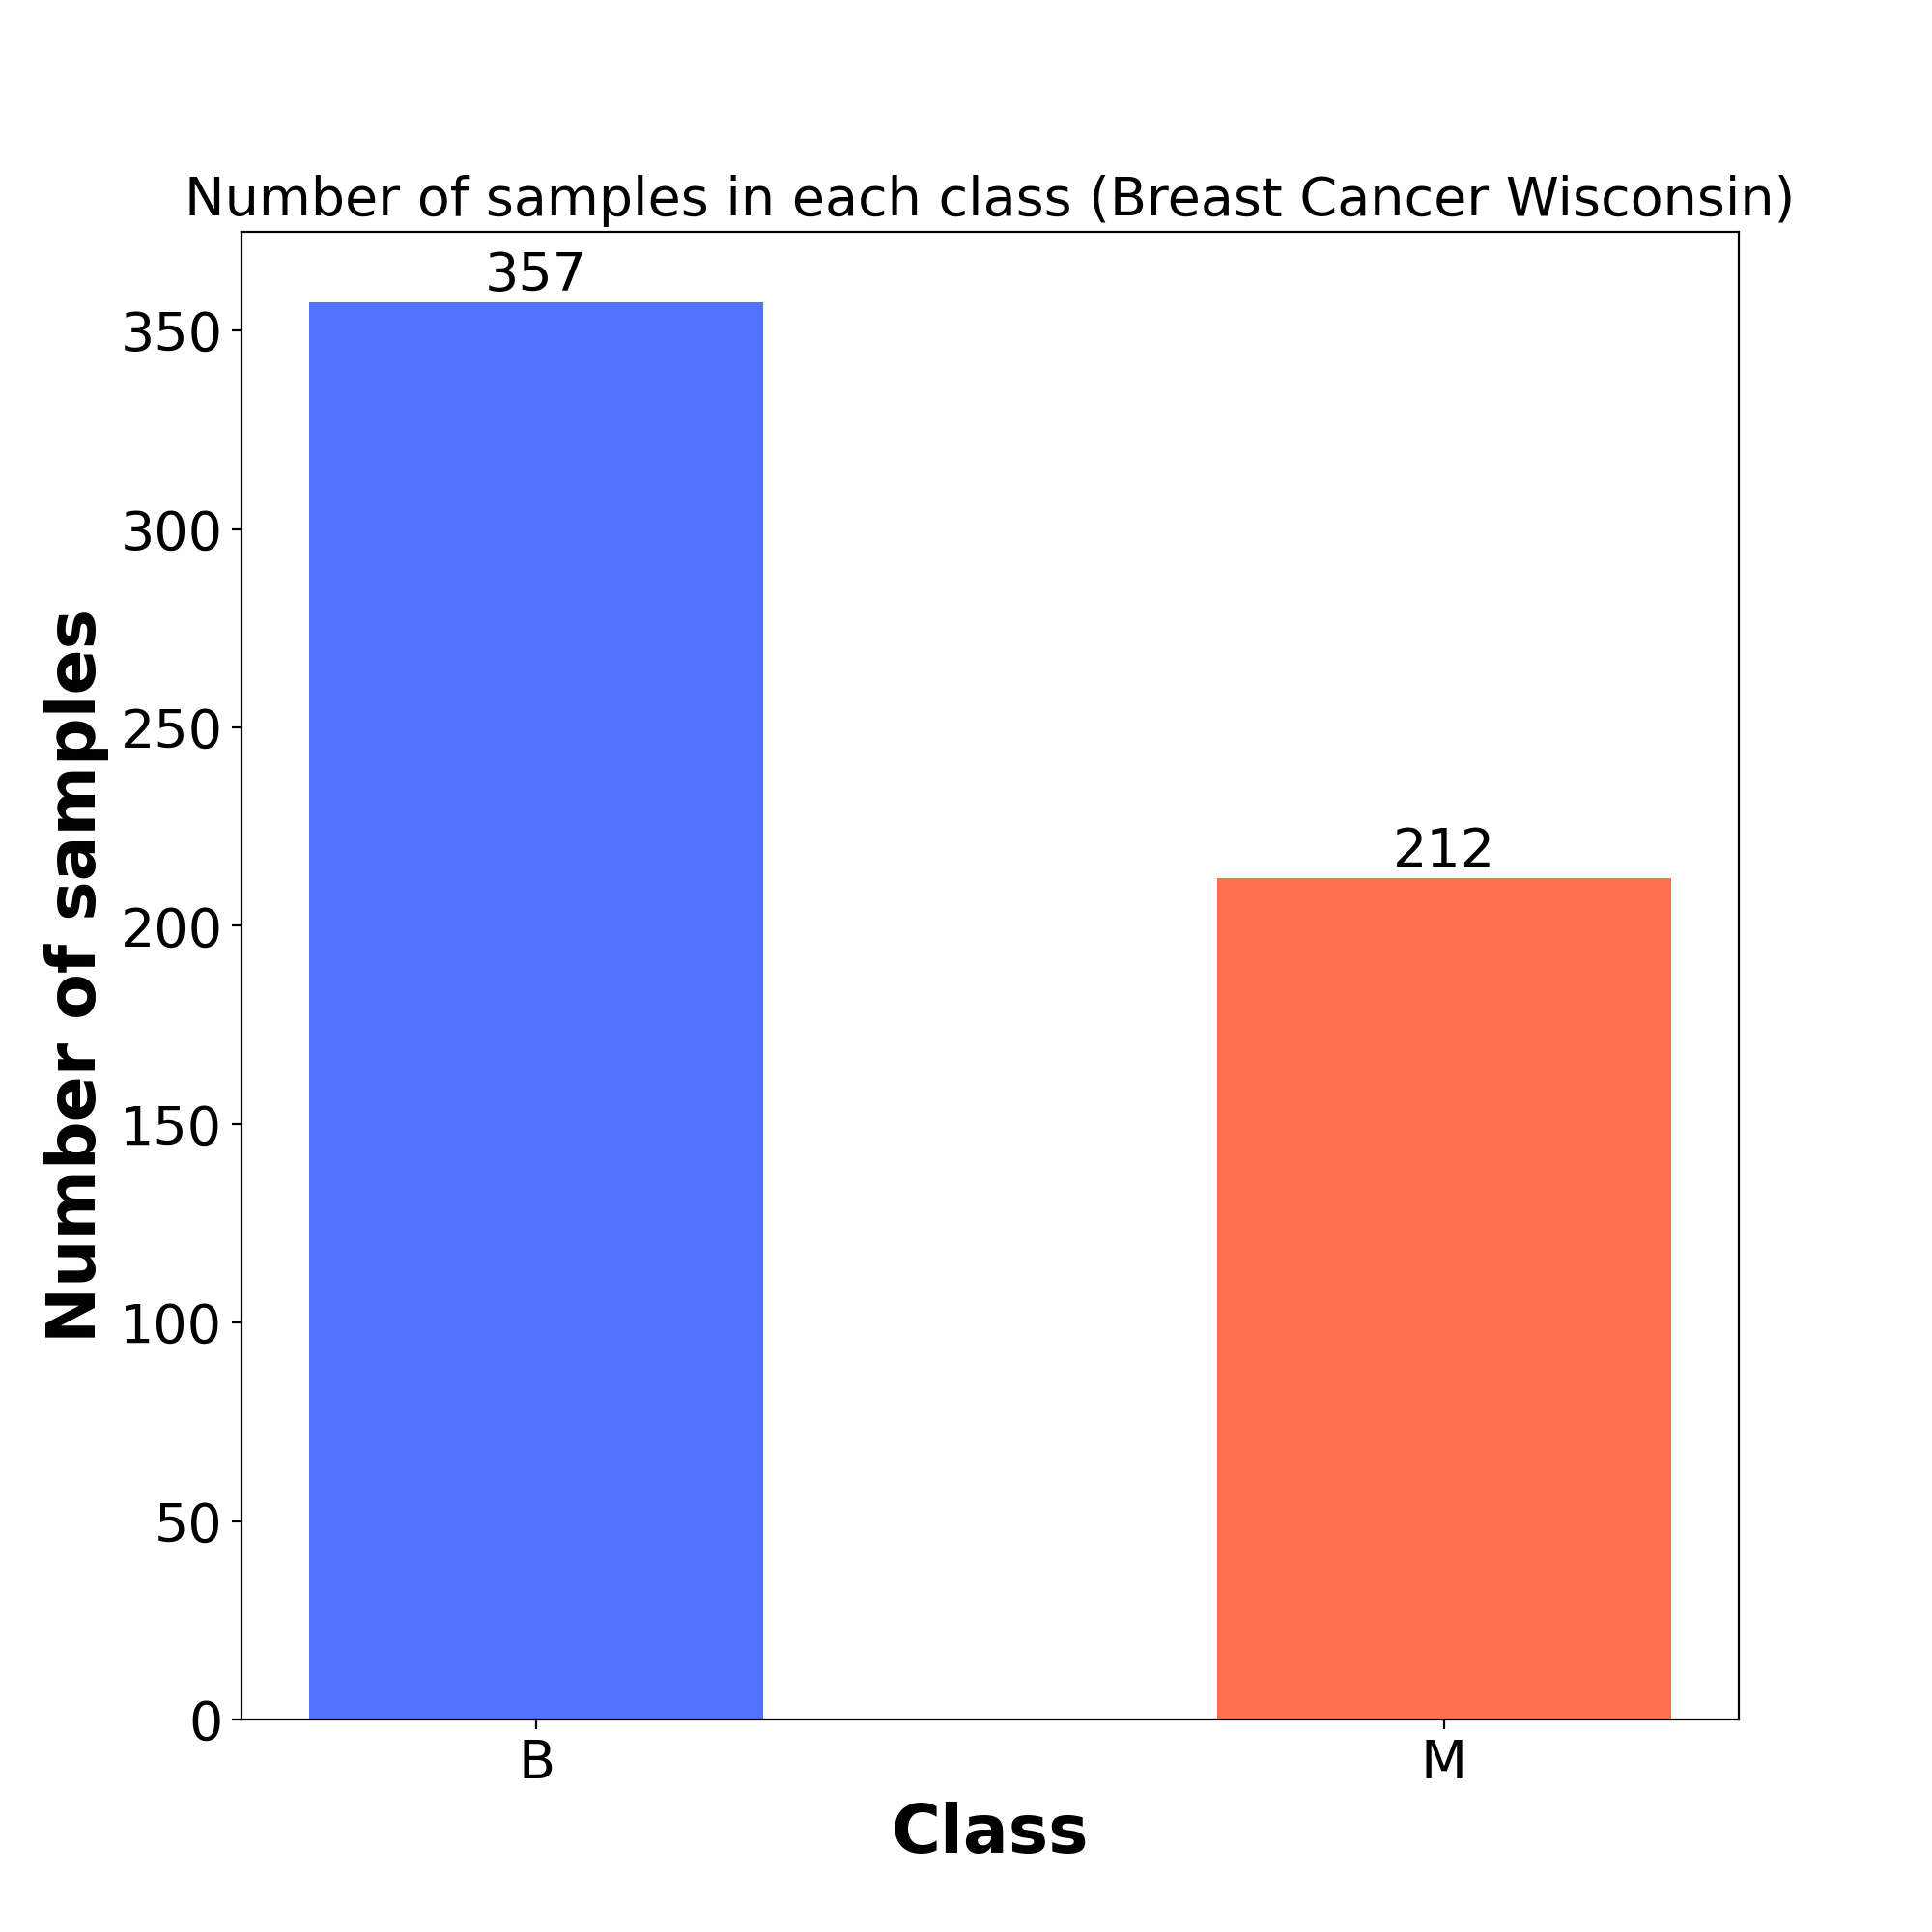
\includegraphics[width=0.7\textwidth]{images/sample/breast_cancer.png}
    \caption{\# Samples for each class of \textit{Breast Cancer Wisconsin} dataset.}
    \label{sbreast}
\end{figure}

\vspace{10pt}

\noindent This dataset is available through Kaggle:

\noindent \url{https://www.kaggle.com/datasets/uciml/breast-cancer-wisconsin-data}
\vspace{10pt}

\noindent This database is also available through the UW CS FTP server:

\noindent ftp: ftp.cs.wisc.edu

\noindent cd math-prog/cpo-dataset/machine-learn/WDBC/
\vspace{10pt}

\noindent Also can be found on the UCI Machine Learning Repository:

\noindent \url{https://archive.ics.uci.edu/ml/datasets/Breast+Cancer+Wisconsin+%28Diagnostic%29}


\subsection{Iris dataset}

The \textit{Iris} dataset is a well-known dataset used by biologist Ronald Fisher (1936) in his paper The use of multiple measurements in taxonomic problems as an example of linear discriminant analysis~\cite{iris}. The dataset contains three iris species as classes: “Iris-setosa,” “Iris-virginica,” and “Iris-versicolor,” with 50 samples each. The dataset has four features for each sample:

\begin{itemize}
\item length of the sepals (range: 4.3cm – 7.9cm)
\item width of the sepals (range: 2.0cm – 4.4cm)
\item length of the petals (range: 1.0cm – 6.9cm)
\item width of the petals (range: 0.1cm – 2.5cm)
 \end{itemize}

Since the range difference of the \textit{Iris} dataset’s features differs from each other when we take the feature difference between prototypes and the samples, we will see the biggest contribution to the distance comes from the length of the petals. Hence the decision mostly relies on the length of the petals because the length of the petals has the highest range difference between the features. We use normalization on the dataset’s features to eliminate the unequal decision power between the features.

 Number of samples for each class in the dataset is given in Figure~\ref{siris}.

\begin{figure}[H]
    \centering
    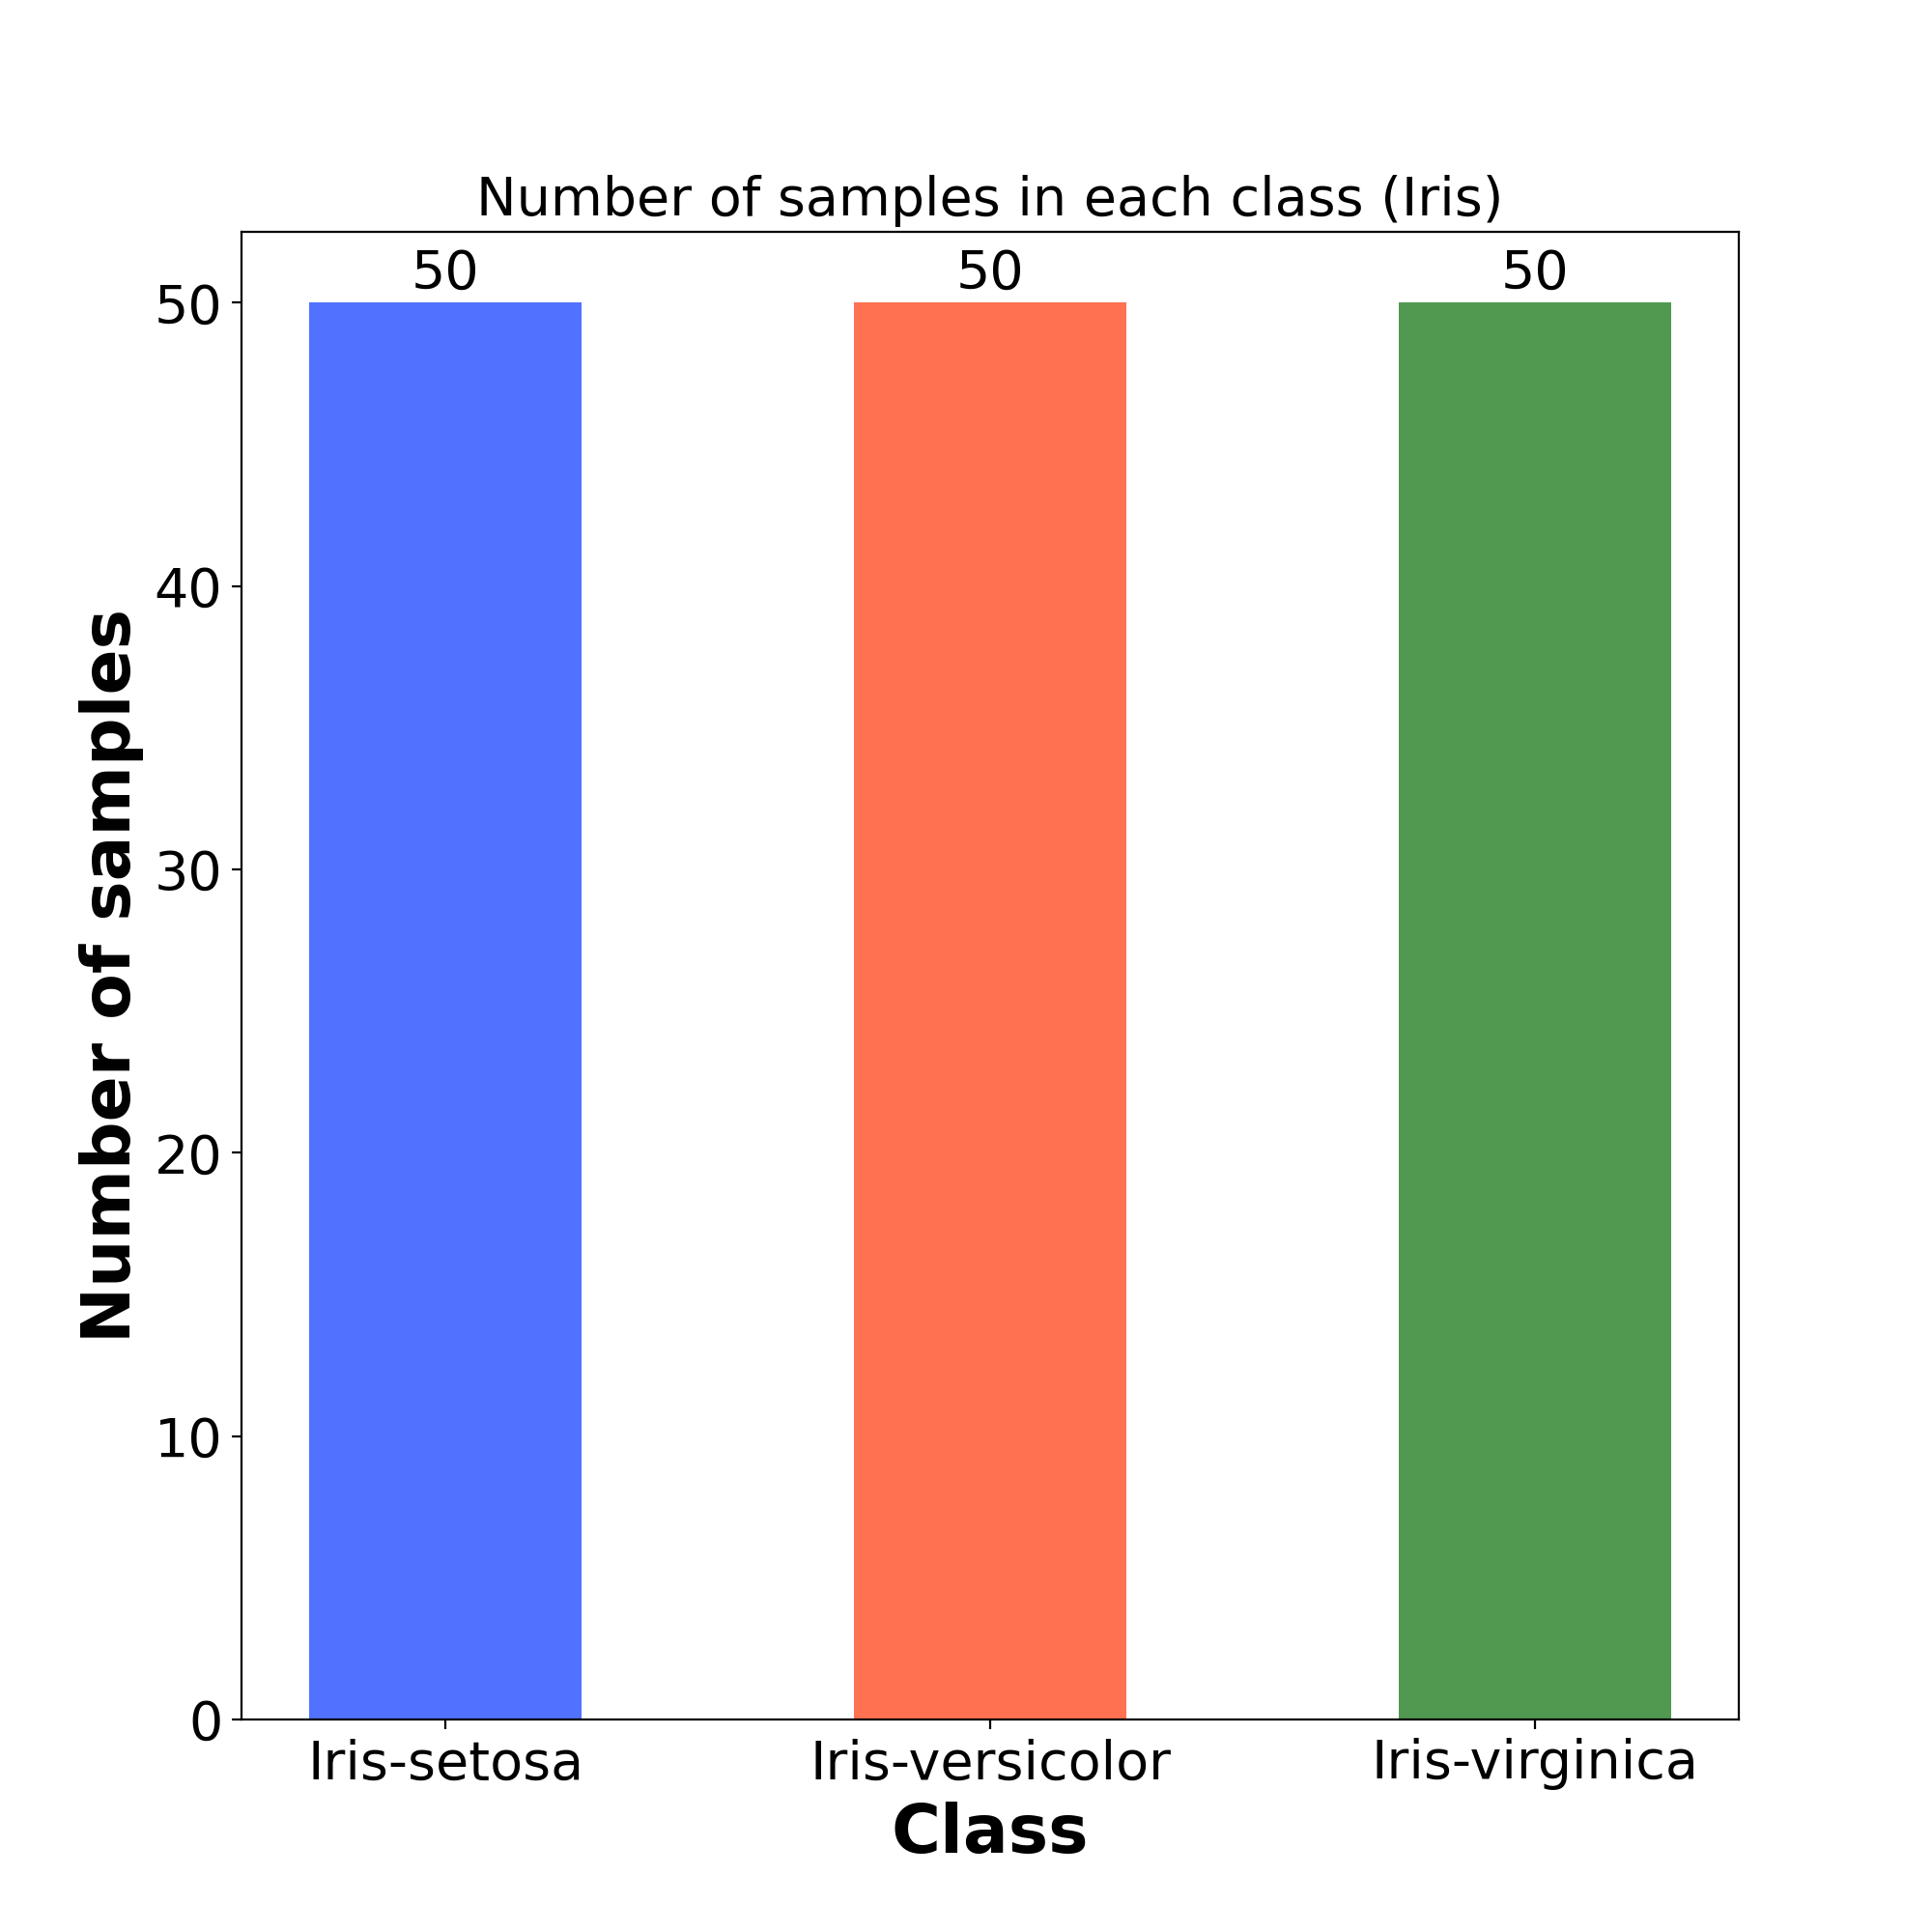
\includegraphics[width=0.7\textwidth]{images/sample/iris.png}
    \caption{\# Samples for each class of \textit{Iris} dataset.}
    \label{siris}
\end{figure}
\vspace{10pt}

\noindent This dataset is available through Kaggle:

\noindent \url{https://www.kaggle.com/datasets/sims22/irisflowerdatasets}

\subsection{Ionosphere dataset}

The \textit{Ionosphere} dataset is donated by Vince Sigillito and sourced by Space Physics Group, Applied Physics Laboratory at Johns Hopkins University. The data is created by measuring the ionosphere to see if there are any free electrons in the ionosphere or not. The data is binary classification with “Good” (G) and “Bad” (B) as class names. “Good” indicates there is evidence that there is some type of structure in the ionosphere, and “Bad” shows there is no structure. The feature size is 34, and there are 351 samples in the \textit{Ionosphere} dataset. Features are signals generated by 16 high-frequency antennas with total transmitted power on the order of 6.4~\cite{ion}. In Figure~\ref{sion} we see the sample distribution of the dataset.

\begin{figure}[H]
    \centering
    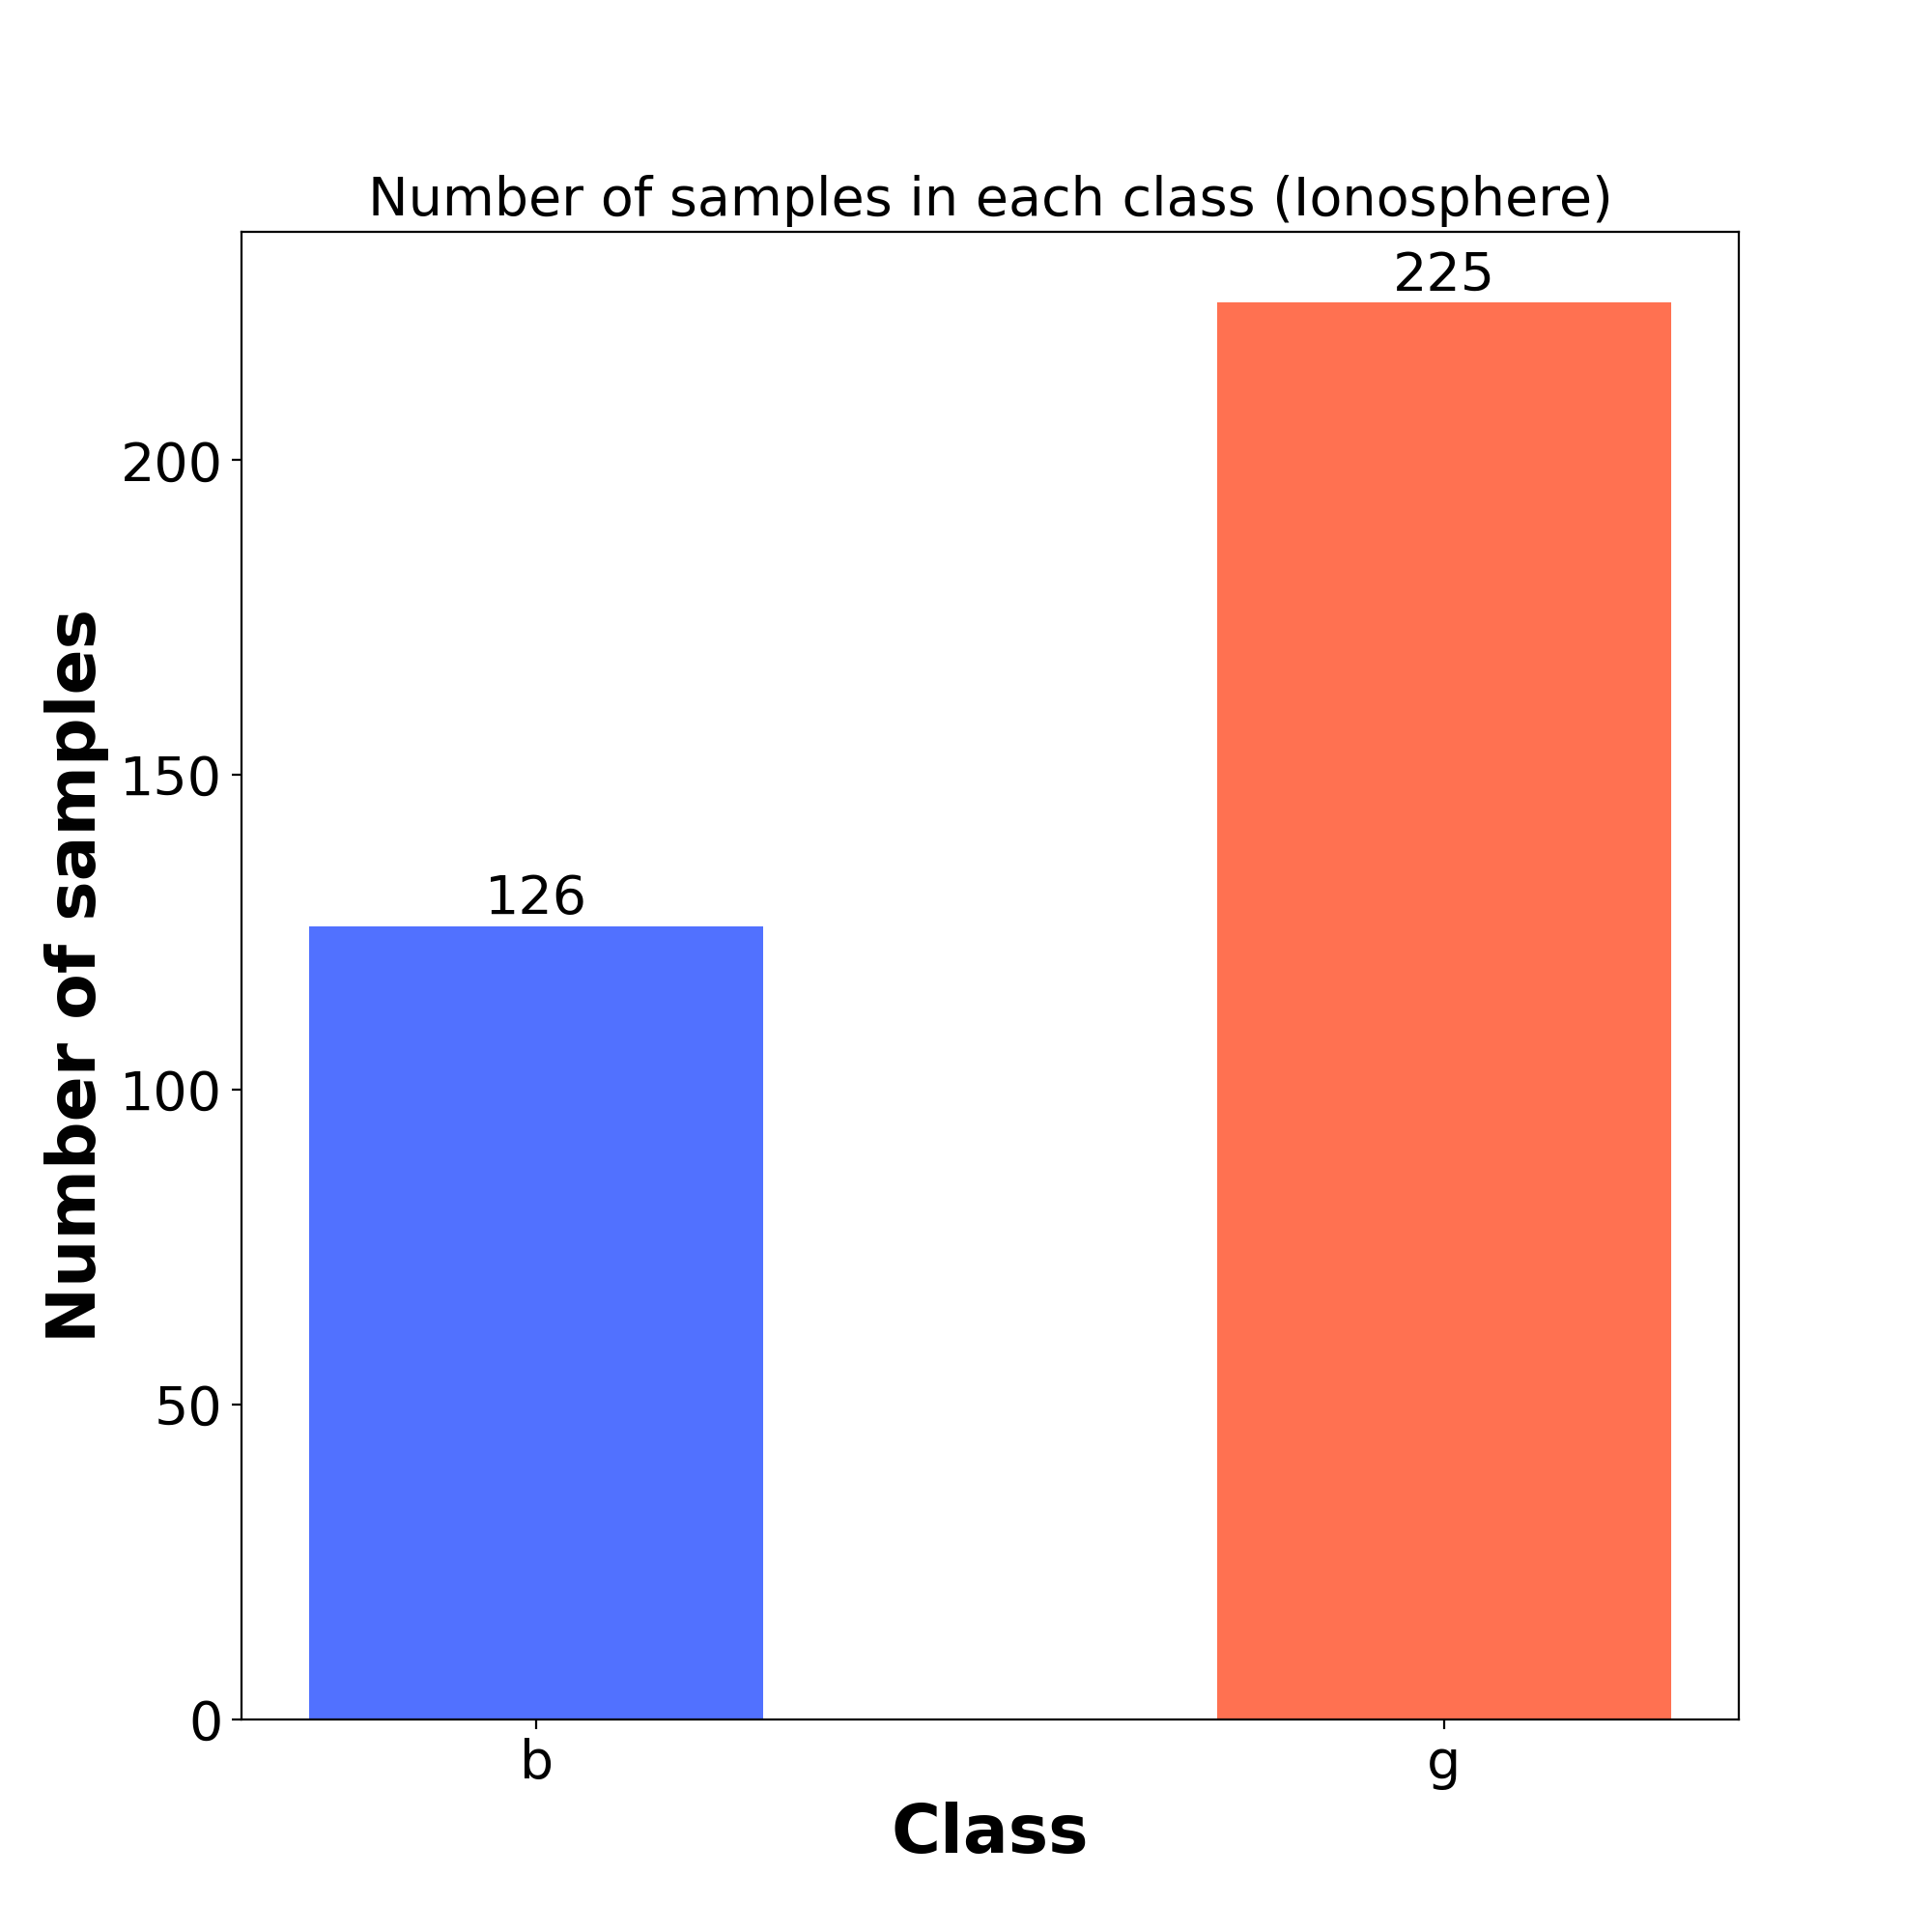
\includegraphics[width=0.7\textwidth]{images/sample/ionosphere.png}
    \caption{\# Samples for each class of \textit{Ionosphere} dataset.}
    \label{sion}
\end{figure}
\vspace{10pt}

\noindent This dataset is available through Kaggle:

\noindent \url{https://www.kaggle.com/datasets/prashant111/ionosphere}
\vspace{10pt}

\noindent Or through UC Irvine Machine Learning Repository:

\noindent \url{https://archive.ics.uci.edu/dataset/52/ionosphere}


\subsection{Sonar dataset}

The \textit{Sonar} is created by Terry Sejnowski at the Salk Institute and the University of California at San Deigo with the collaboration of R. Paul Gorman of Allied-Signal Aerospace Technology Center~\cite{sonar}, and the dataset is used in the study “Analysis of Hidden Units in a Layered Network Trained to Classify Sonar Targets.” \textit{Sonar} dataset contains sonar signals bouncing off metal cylinders of “Mines” (M) and “Rocks” (R) under various angles and conditions~\cite{sonar}. The dataset contains 111 “Mines” and 97 “Rocks” samples. Each sample contains 60 features in the range between $0.0$ and $1.0$, representing the energy in a particular frequency band. In their experiment, Gorman, R. P., and Sejnowski, T. J. achieved accuracy between $77.1\%$ and $90.4\%$ on a test set using neural networks varying between 0 to 24 hidden layers~\cite{sonar}. Figure~\ref{ssonar} shows the sample distribution of the \textit{Sonar} dataset.

\begin{figure}[H]
    \centering
    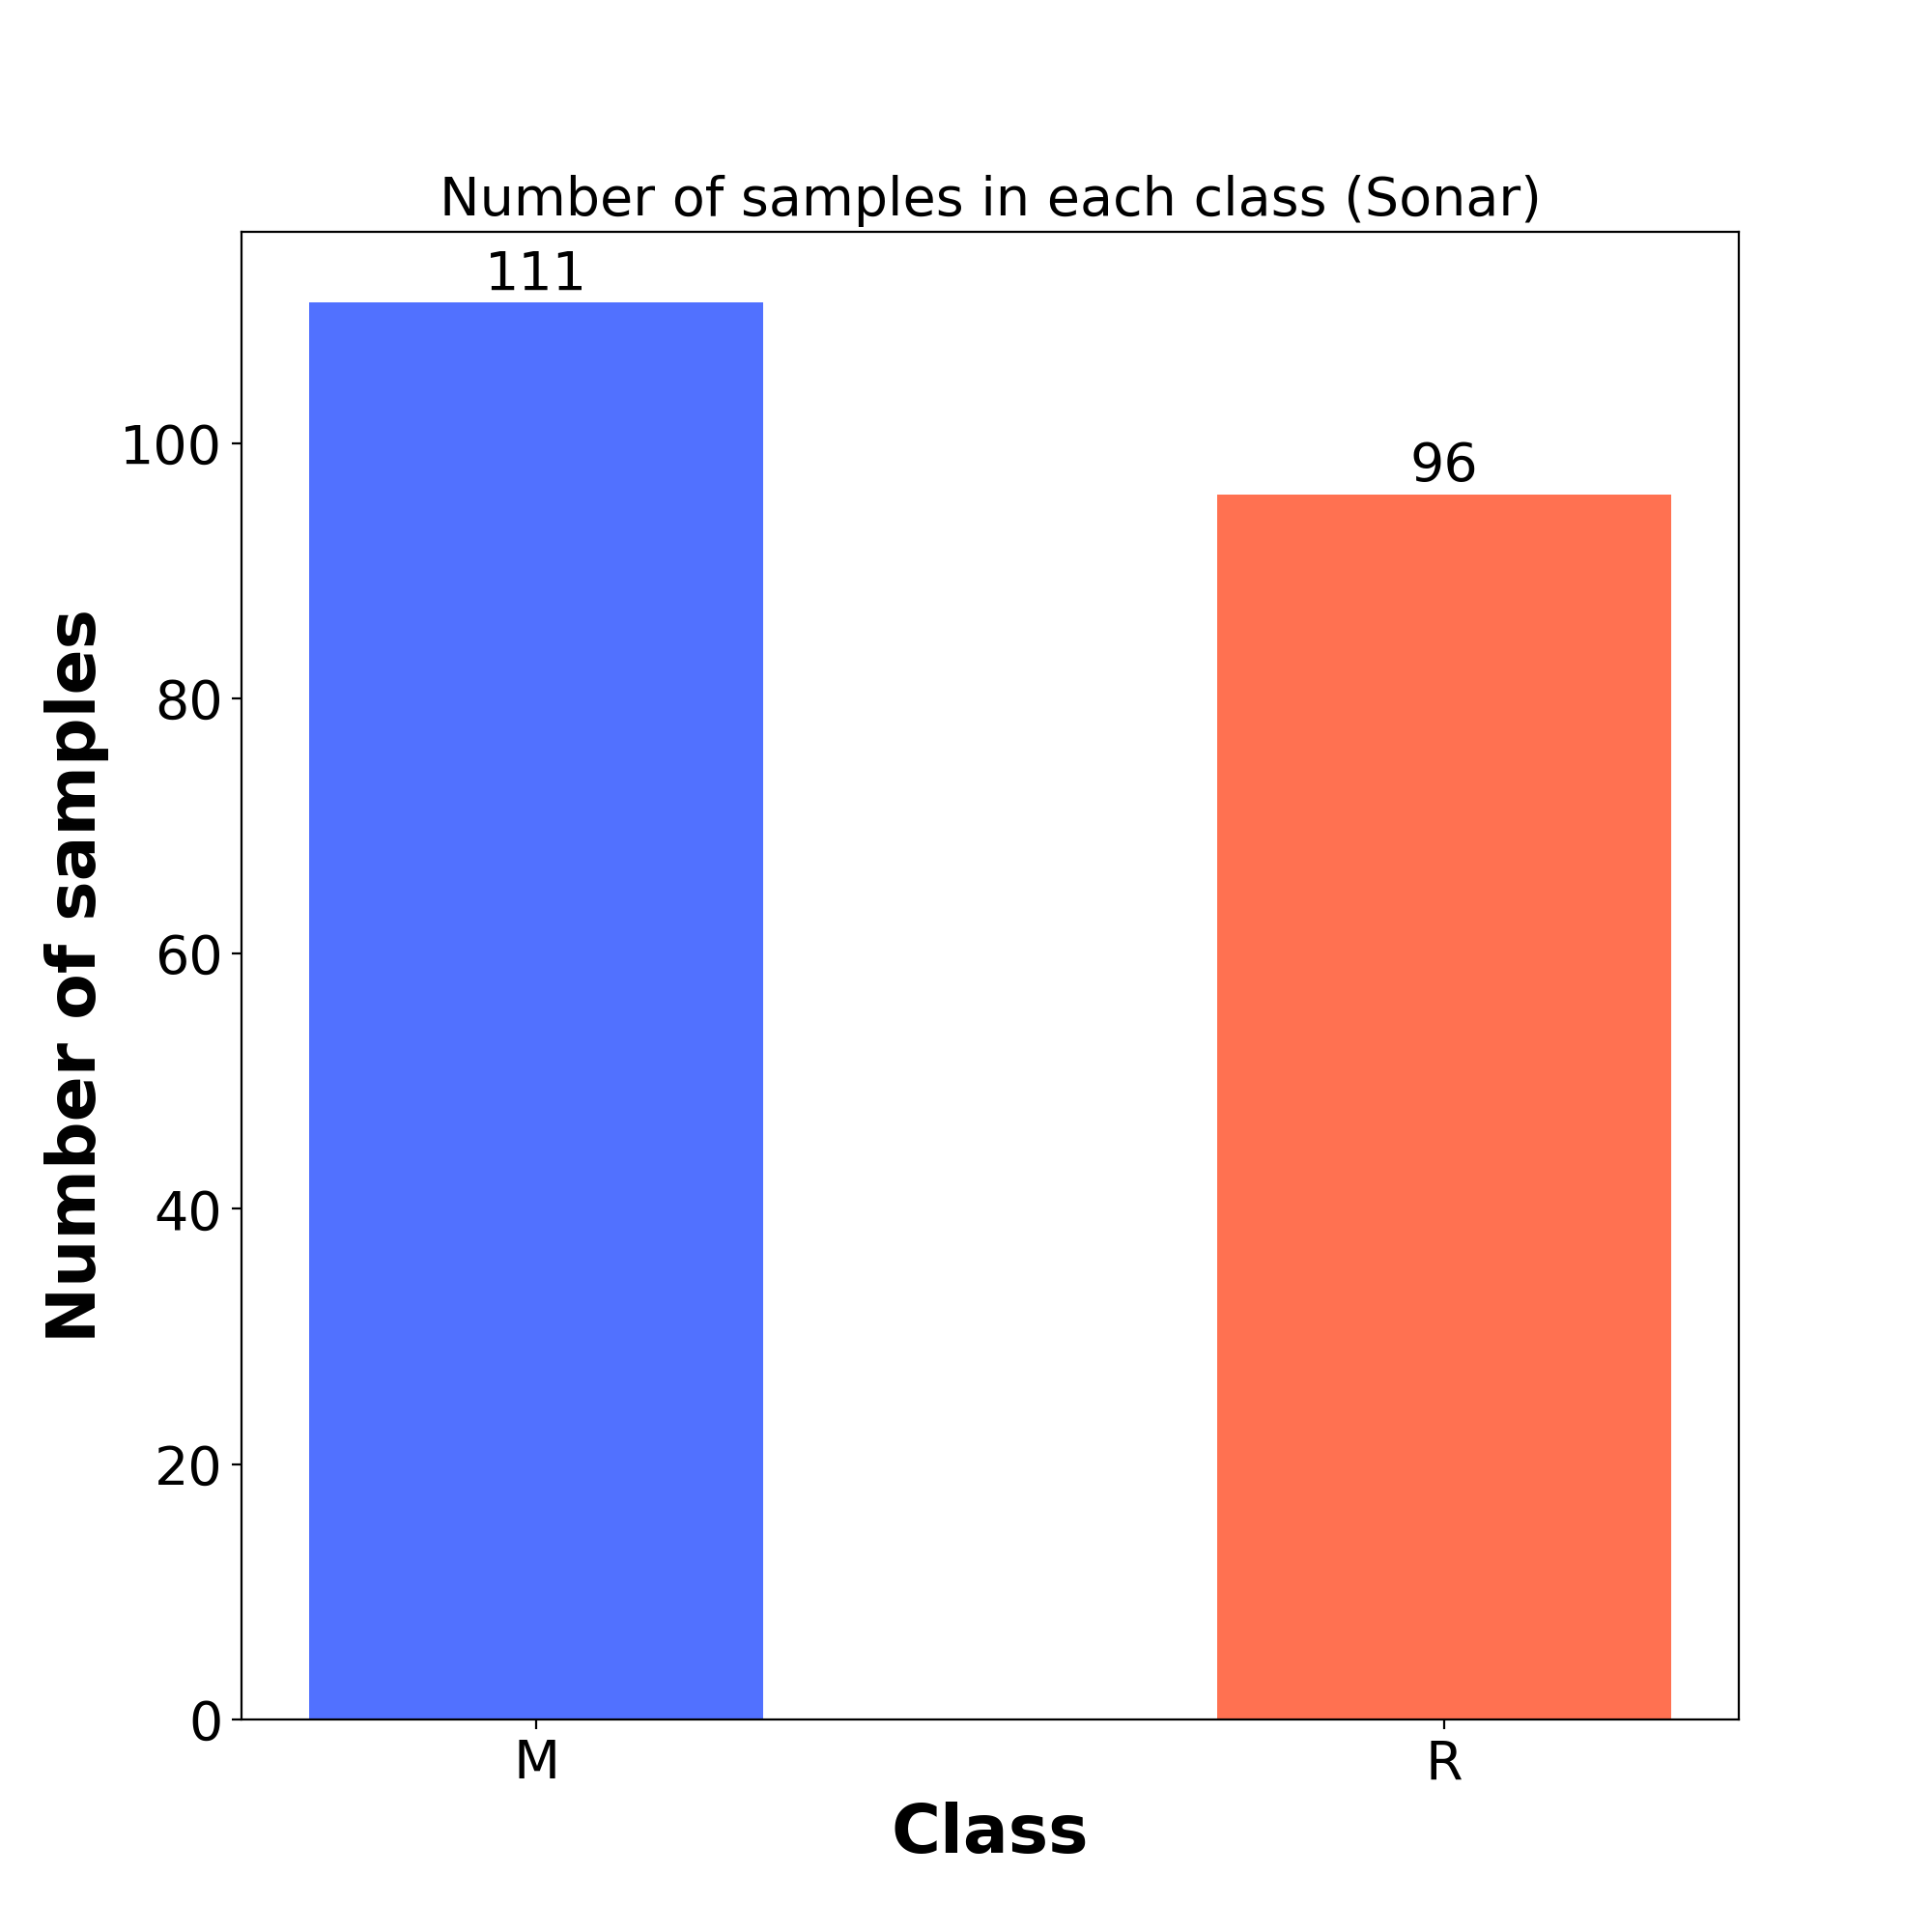
\includegraphics[width=0.7\textwidth]{images/sample/sonar.png}
    \caption{\# Samples for each class of \textit{Sonar} dataset.}
    \label{ssonar}
\end{figure}
\vspace{10pt}

\noindent This dataset is available through Kaggle:

\noindent \url{https://www.kaggle.com/datasets/rupakroy/sonarcsv}


\subsection{SP and NSP datasets}

Besides open-source datasets, our private datasets were created from the IFE blood test data we mentioned in the Section~\ref{creIFE}. The first dataset we created from IFE test data takes the Fourier transforms of all the bars, including SP bars, and groups the samples into “Normal” and “Abnormal” classes. Every group except “wo” and “ud” is labeled “Abnormal,” and “wo” data turns into “Normal.” We do not take into account undefined data. While selecting prototypes for this dataset, we first select the prototypes from each sick group and then join them. We select one prototype from the “Normal” class for each “Abnormal” class prototype. The prototypes selected from the “Abnormal” class are divided equally by every group contributing to the class. Figure~\ref{sife1} shows the sample number of each class before grouping the labels into two groups, while Figure~\ref{sife2} shows the sample number of each class after labeling the classes into two groups, “Normal” and “Abnormal.”

\begin{figure}[H]
    \centering
    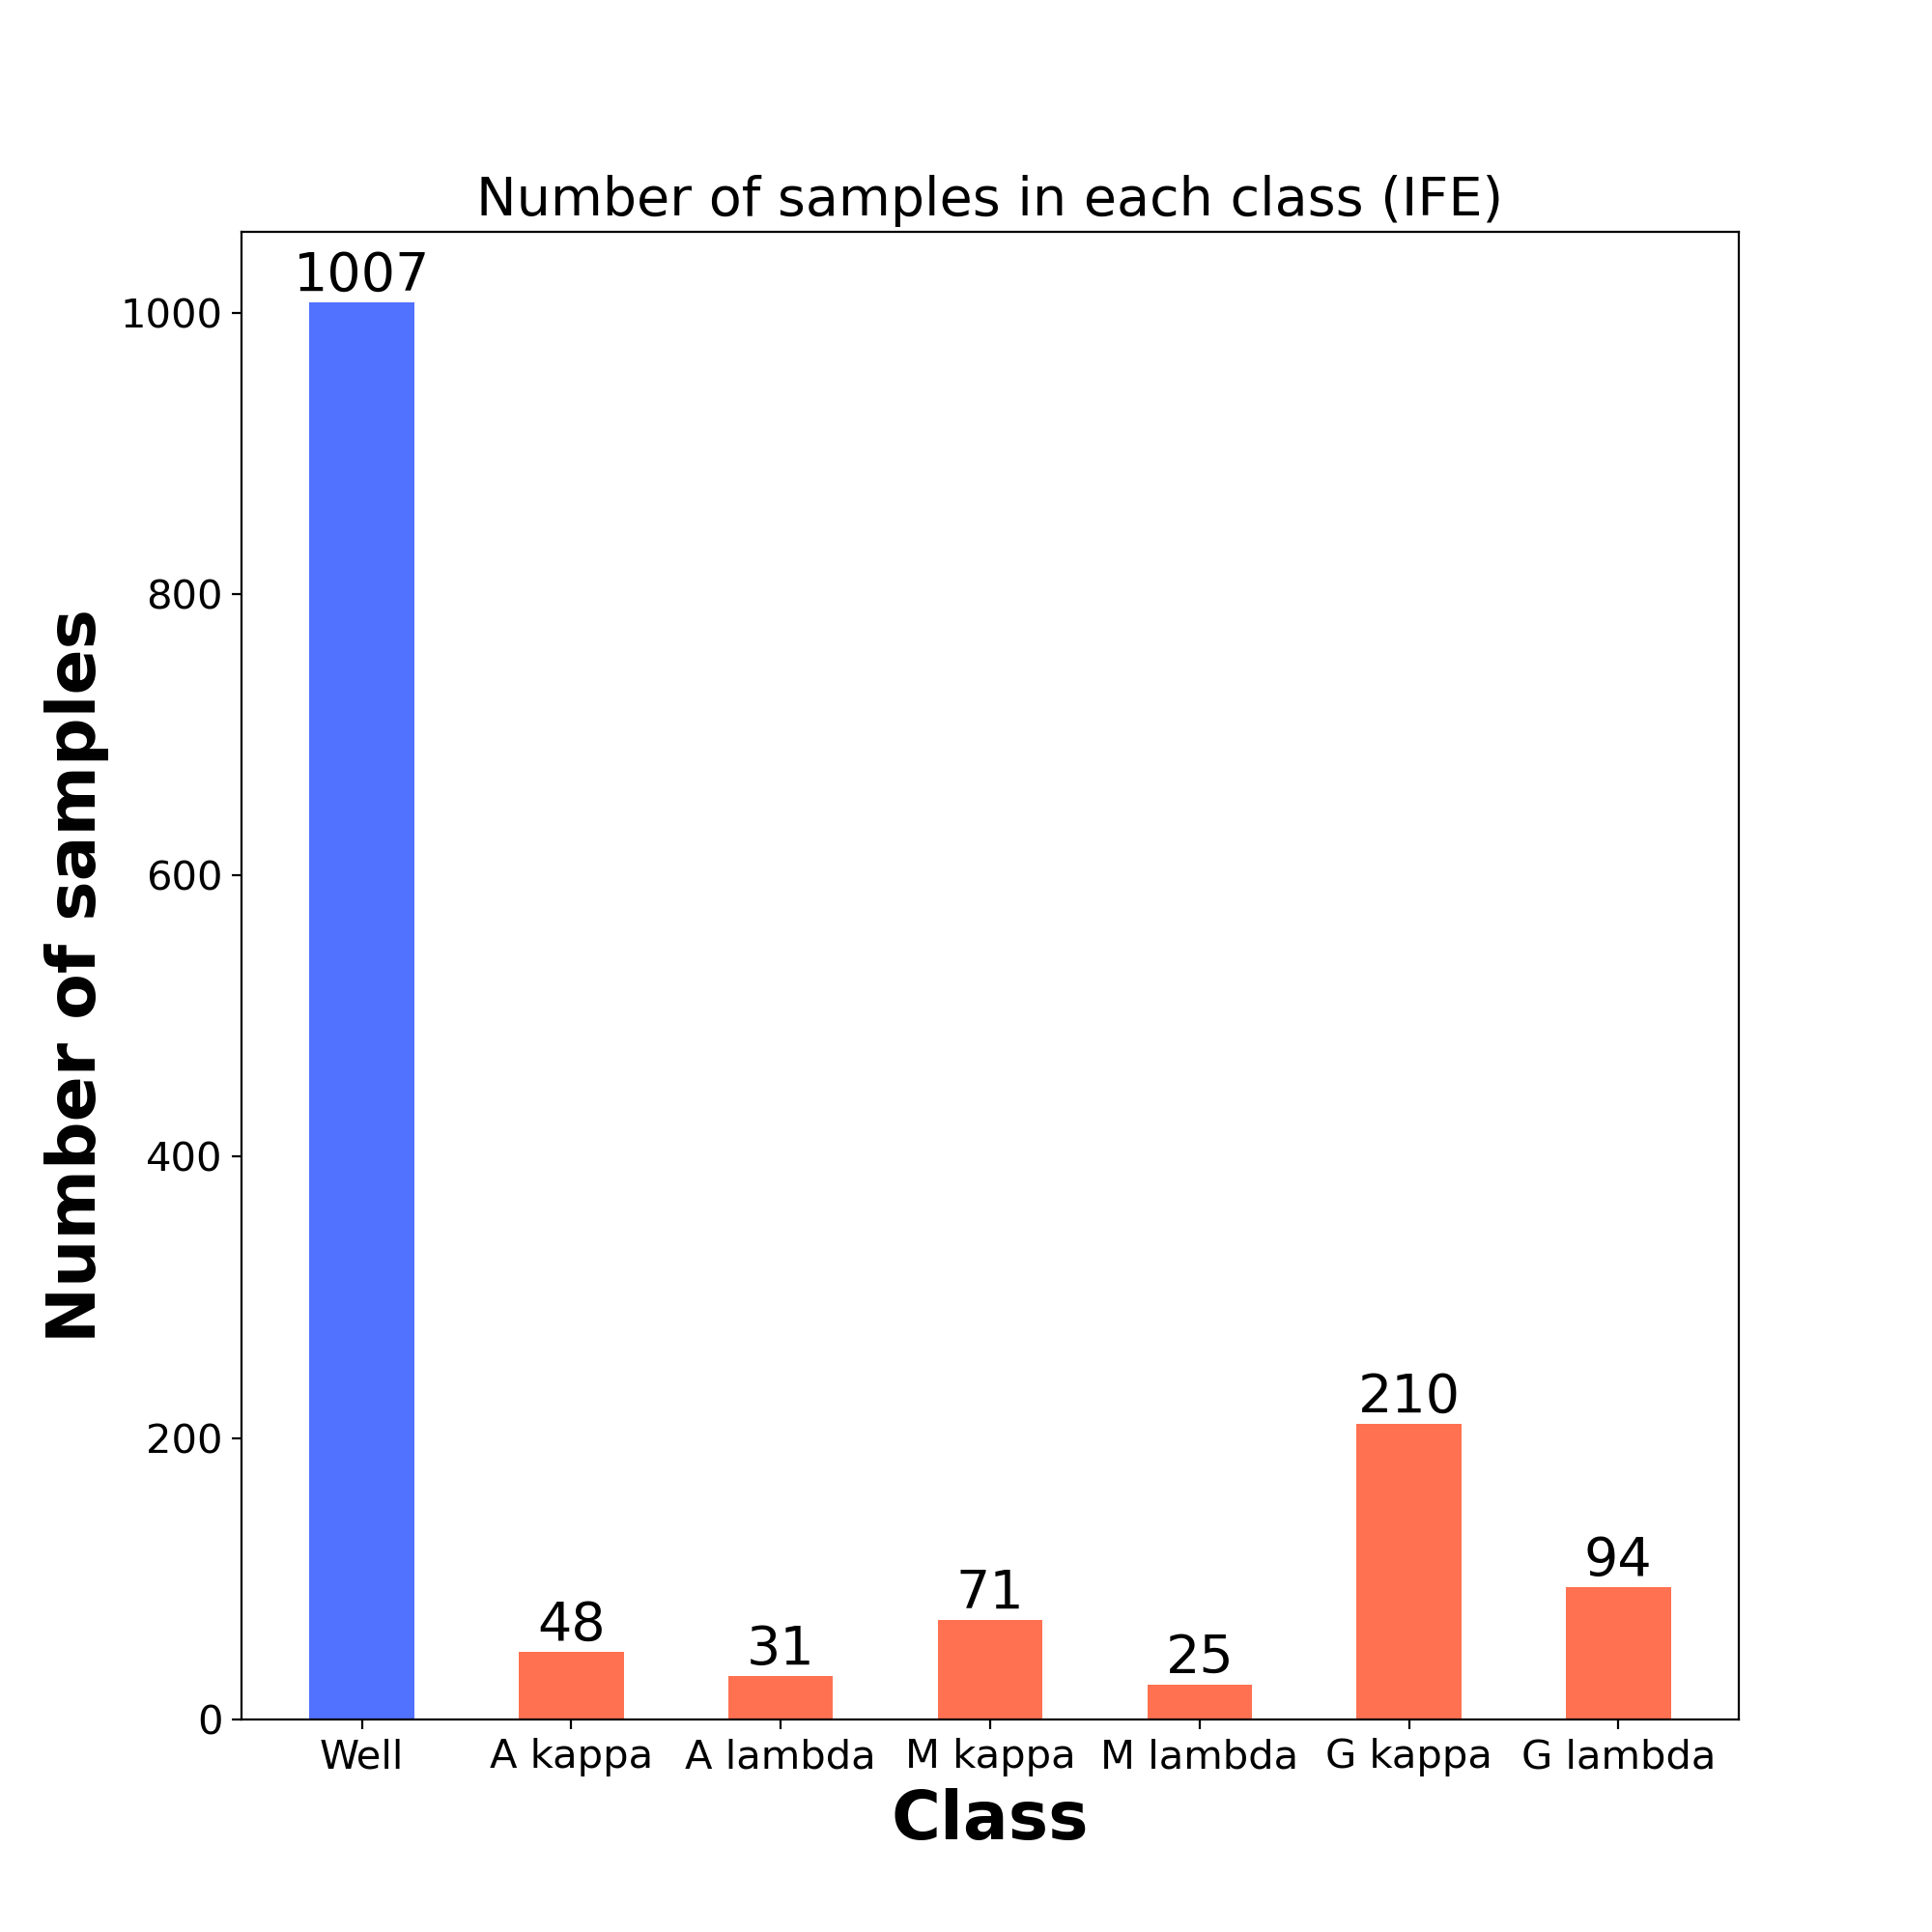
\includegraphics[width=0.7\textwidth]{images/sample/IFE_1.png}
    \caption{\# Samples for each class of \textit{SP and NSP} dataset.}
    \label{sife1}
\end{figure}

\begin{figure}[H]
    \centering
    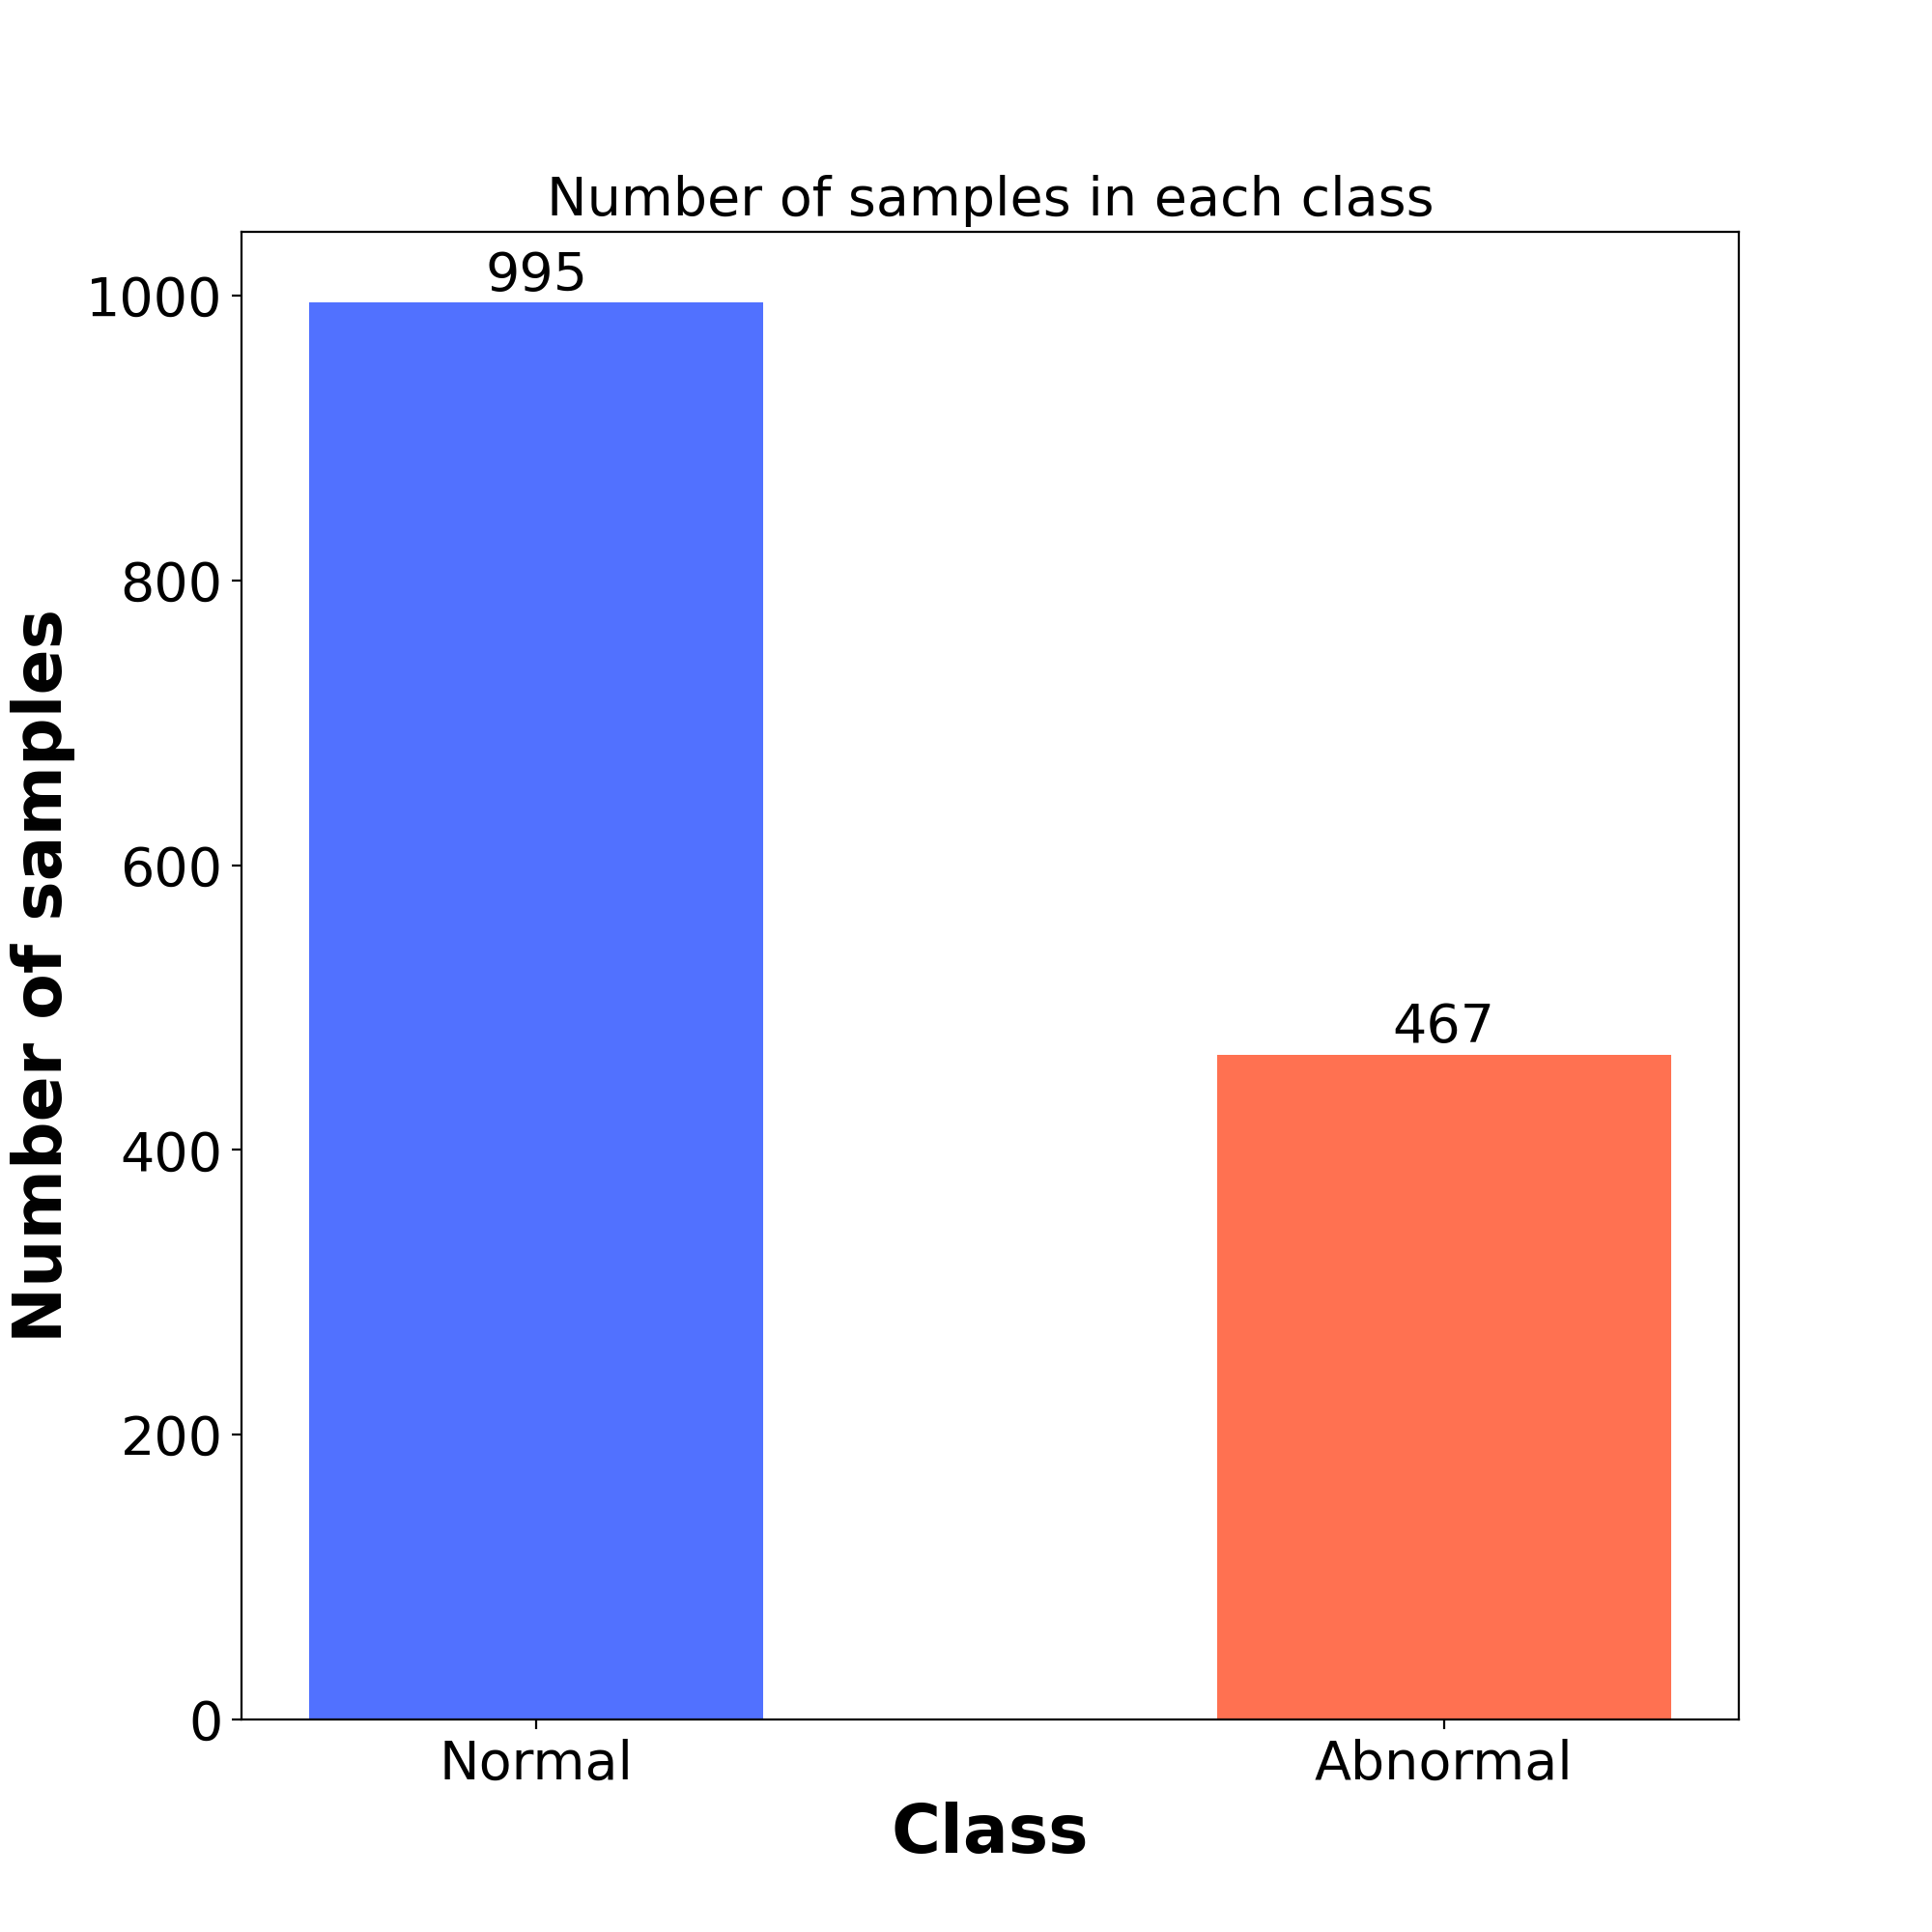
\includegraphics[width=0.7\textwidth]{images/sample/IFE_2.png}
    \caption{\# Samples for each class of \textit{SP and NSP} dataset after grouping classes into two groups.}
    \label{sife2}
\end{figure}

The second dataset we created from IFE test data takes all the bars except the SP bar while applying the Fourier transform. We apply the same logic to the first dataset we created from IFE test data and divide the samples into “Normal” and “Abnormal” classes. Since each bar on IFE data has a length of 184 pixels (values), while the \textit{SP} dataset has 1104 entries as a feature-length for each sample, \textit{NSP} dataset has 920 entries. Both of the created IFE datasets have the same sample size of 1486 samples. We use the Fourier transform in both IFE datasets since the bars of IFE blood samples are examined by the coloration (frequency) change rather than the coloration value.


\section{Models}

\subsection{GLVQ}

There are many LVQ sub-models, but all the sub-models have the same principle: all prototype-based supervised learning algorithms. In a prototype-based algorithm, we use no weight vectors but prototypes ($\omega$), a small group of our data. When we train the model, the prototypes move closer or farther away from the trained data depending on the situation and the sub-model. Ultimately, the distance of features of the sample from the selected prototypes’ final values makes the decision. Since we use GLVQ (Generalized LVQ)~\cite{sato} as the sub-model of LVQ in this paper, we first explain the construct of GLVQ.

GLVQ has been coined out by Sato and Yamada (1995)~\cite{sato}. As with all the other LVQ models, GLVQ has prototypes with classes and local learning rates for each $\omega$. First, we set the initial learning rate ($\epsilon(0)$), which (de)amplifies the prototypes’ movement speed to the given direction. Learning rate at time $t$ ($\epsilon(t)$) changes depending on the current state of the $\omega$ and prediction. We use different types of learning rate updates for different learning rate update approaches. Each $\omega_{i}$ can have different $\epsilon$, namely local $\epsilon$ ($\epsilon_{i}$), which makes each $\omega$ learn on a different scale.

After choosing our $\epsilon(0)$, we must choose our prototypes. Prototypes must include all the class types. If one of the class representatives would be missing, then we would not have a prediction for the given class. We measure the distance between each training sample and all the prototypes. Generally, squared Euclidian distances are used for the distance measurement for LVQ. The Equation~\eqref{distr} shows squared Euclidian distance with real-valued arrays. When we transform data with Fourier transform, data become complex-valued inputs. The calculation we use is still squared Euclidian distance for complex values, which is the Equation~\eqref{distc}, where $\mathbb{x}^{c}\in \mathbb{C}^{n}$ is a complex-valued array with $\mathbb{x}^{c} = a + i\cdot b$, where $a,b\in\mathbb{R}^{n}$.

\begin{itemize}
\item $n$: number of features in $\mathbb{x}$
\item $x_{i}$: $i^{\text{th}}$ feature value of $\mathbb{x}$
\item $y_{i}$: $i^{\text{th}}$ feature value of $\omega_{j}$
\item $d_{r}(\mathbb{x},\omega_{j})$: distance for real values between $\mathbb{x}$ and $\omega_{j}$ features
\item $d_{c}(\mathbb{x}^{c},\omega_{j}^{c})$ distance for complex values between $\mathbb{x}$ and $\omega_{j}$ features
\end{itemize}
Then:
\vspace{10pt}

\begin{subequations}
\label{dists}
\renewcommand{\theequation}{\theparentequation.\arabic{equation}}
    \begin{equation}
d_{r}(\mathbb{x},\omega_{j}) = \sum_{i=1}^{n} (x_{i} - y_{i})^{2}\label{distr}
    \end{equation}
   \begin{equation}
d_{c}(\mathbb{x}^{c},\omega_{j}^{c}) = \sum_{i=1}^{n} (|x^{c}_{i} - y^{c}_{i}|^{2})\label{distc}
   \end{equation}
    \end{subequations}
\vspace{10pt}

GLVQ has two winner $\omega$, and both are updated. The first winner is the closest $\omega$ to the sample $\mathbb{x}$ with the same class with distance noted as $d^{+}(\mathbb{x})$, and the second winner is the closest $\omega$ to the sample with a different class with distance noted as $d^{-}(\mathbb{x})$. We can define a $\mu(\mathbb{x})$ of sample array $\mathbb{x}$ as a relative distance in Equation~\eqref{mu}. According to Sato and Yamada (1995), when the $\mu(\mathbb{x})$ value for $\mathbb{x}$ is negative, the prediction is correct and false otherwise~\cite{sato}.
\vspace{10pt}

\begin{equation}
\mu(\mathbb{x}) = \frac{d^{+}(\mathbb{x}) - d^{-}(\mathbb{x})}{ d^{+}(\mathbb{x}) + d^{-}(\mathbb{x})}\label{mu}
\end{equation}
\vspace{10pt}


 $\mu(\mathbb{x})$ calculation is used in cost function ($S$) like in the Equation~\eqref{cost} to calculate the error of the model’s current state. Error is used to update the model to a local minimum error state by using the derivative of $S$ with $N\in\mathbb{N}$ samples.
\vspace{10pt}


\begin{equation}
S = \sum_{\forall i \in N}f(\mu(\mathbb{x}_{i}))\label{cost}
\end{equation}
\vspace{10pt}


To use $\mu(\mathbb{x})$ in $S$, first $\mu(\mathbb{x})$ must go under an activation function $f$ (which is primarily the Sigmoid function ($\sigma$) in the Equation~\eqref{sigma}). The winners updated in the direction of the sample with amplitude of the $\epsilon(t)$ and $\partial S$.
\vspace{10pt}


\begin{equation}
\sigma(\mu(\mathbb{x})) = \frac{1}{1 + e^{-\mu(\mathbb{x})}}\label{sigma}
\end{equation}
\vspace{10pt}


The first winner $\omega$ ($\omega^{+}$) is updated by the attraction in the Equation~\eqref{w1}, while we apply repulsion on the second winner ($\omega^{-}$) in the Equation~\eqref{w2}~\cite{sato}. These calculations come from $\frac{\partial S}{\partial \omega}$. Attraction makes $\omega^{+}$ move closer to the given sample by its local $\epsilon$ value, $\epsilon^{+}$; while repulsion makes the $\omega^{-}$ move further away from the sample with $\epsilon^{-}$. This way, next time, $\omega^{+}$ would have a better chance to be the winner for the same sample while $\omega^{-}$ would have less chance to be the winner.
\vspace{10pt}

\begin{subequations}
\label{w updates}
\renewcommand{\theequation}{\theparentequation.\arabic{equation}}
\noindent Attraction:
    \begin{equation}
   \omega^{+}(t+1) = \omega^{+}(t) - \epsilon^{+}\frac{\partial S}{\partial \omega^{+}}\label{w1}
   \end{equation}
Repulsion:
\begin{equation}
   \omega^{-}(t+1) = \omega^{-}(t) - \epsilon^{-}\frac{\partial S}{\partial \omega^{-}}\label{w2}
\end{equation}
    \end{subequations}
\vspace{10pt}

The OGLVQ model and CGLVQ models are structured above the GLVQ model.




\subsection{Learning rate optimizers}

We use GLVQ to create a more human-like learning system for the learning algorithm. A component in every machine learning algorithm is the $\epsilon$, which controls the learning speed of each training sample. Taking the $\epsilon(0)$ high might seem reasonable to create a fast learning machine learning method, but the reality is far away from that. A high $\epsilon(0)$ causes the method to fixate on the last training sample, which would diminish the knowledge learned from the previous training samples. On the other hand, if the $\epsilon(0)$ is too low, there would be no learning from the training set. That is why we need to find an adequate $\epsilon(0)$ with optimal learning rate update for the method since an optimal $\epsilon$ gives a better prediction. For this paper, we use the optimized learning rate method for GLVQ from Kohonen (1995)~\cite{kohonen1} and learning rate methods from cognitive science~\cite{els,cogn,lrimp}.


\subsubsection{Optimized GLVQ}

We use an Optimized Learning Rate on GLVQ as a basis for our experiments. In the book “Self-Organizing Maps” by Kohonen (1995)~\cite{kohonen1}, the schema of OLVQ1 is given, but we implement only the learning rate part of the GLVQ to construct OGLVQ. The paper explains that the optimal learning rate for LVQ1 comes from the prototype update~\cite{kohonen1}. Assumption here is that when updating $\omega_{i}(t+1)$, $\omega_{i}(t)$ contains trance of $\epsilon_{i}(t-1)$. So to reach the optimal $\epsilon_{i}(t)$, we take the $\omega_{i}(t+1)$ update equation on GLVQ for both of the $\omega$ updates, change the $\omega_{i}(t)$ values with $\epsilon_{i}(t-1)$ and solve the equation for $\epsilon_{i}(t)$. The winner $\omega(t)$ updates for squared distance can be seen in the Equation~\eqref{w1up} and ~\eqref{w2up} respectively for GLVQ under squared Euclidian distance and $\sigma$ as activation function.
\vspace{10pt}


\begin{subequations}
\label{w updates 2}
\renewcommand{\theequation}{\theparentequation.\arabic{equation}}
    \begin{equation}
	\begin{split}
\omega^{+}(t+1) &= \omega^{+}(t) - \epsilon^{+}\cdot \frac{\partial S}{\partial \omega^{+}}\\
\\
&= \frac{\partial S}{\partial\mu}\cdot \frac{\partial\mu}{\partial d^{+}(\mathbb{x})}\cdot \frac{\partial d^{+}(\mathbb{x})}{\partial\omega^{+}}\\
\\
&= \omega^{+}(t) +\epsilon^{+}(t)\cdot \sigma(\mu(\mathbb{x}))\cdot [1-\sigma(\mu(\mathbb{x}))]\cdot \frac{4d^{-}(\mathbb{x})}{[d^{+}(\mathbb{x}) + d^{-}(\mathbb{x})]^{2}}\cdot [\mathbb{x} - \omega^{+}(t)]\label{w1up}
\end{split}
\end{equation}
  \begin{equation}
\begin{split}
\omega^{-}(t+1) &= \omega^{-}(t) - \epsilon^{-}\cdot \frac{\partial S}{\partial \omega^{-}}\\
\\
&= \frac{\partial S}{\partial\mu}\cdot \frac{\partial\mu}{\partial d^{-}(\mathbb{x})}\cdot \frac{\partial d^{-}(\mathbb{x})}{\partial\omega^{-}}\\
\\
&= \omega^{-}(t) -\epsilon^{-}(t)\cdot \sigma(\mu(\mathbb{x}))\cdot [1-\sigma(\mu(\mathbb{x}))]\cdot \frac{4d^{+}(\mathbb{x})}{[d^{+}(\mathbb{x}) + d^{-}(\mathbb{x})]^{2}}\cdot [\mathbb{x} - \omega^{-}(t)]\label{w2up}
\end{split}
    \end{equation}
    \end{subequations}
\vspace{10pt}



To find the optimized learning rate update equation of GLVQ, we use the Equations~\eqref{w1up} and ~\eqref{w2up} to generate The Equations~\eqref{alpha1up} and ~\eqref{alpha2up} respectively.
\vspace{10pt}

\begin{subequations}
\label{alpha updates}
\renewcommand{\theequation}{\theparentequation.\arabic{equation}}
    \begin{equation}
\epsilon^{+}(t) = [1 - \epsilon^{+}(t)]\cdot \sigma(\mu(\mathbb{x}))\cdot [1-\sigma(\mu(\mathbb{x}))]\cdot  \frac{4d^{-}(\mathbb{x})}{[d^{+}(\mathbb{x}) + d^{-}(\mathbb{x})]^{2}}\cdot \epsilon^{+}(t-1)\label{alpha1up}
    \end{equation}
    \begin{equation}
\epsilon^{-}(t) = [1 + \epsilon^{-}(t)]\cdot \sigma(\mu(\mathbb{x}))\cdot [1-\sigma(\mu(\mathbb{x}))]\cdot  \frac{4d^{+}(\mathbb{x})}{[d^{+}(\mathbb{x}) + d^{-}(\mathbb{x})]^{2}}\cdot \epsilon^{-}(t-1)\label{alpha2up}
    \end{equation}
    \end{subequations}
\vspace{10pt}

At the end, if we re-arrange the Equations~\eqref{alpha1up} and ~\eqref{alpha2up} for $\epsilon(t)$, the OGLVQ $\epsilon(t)$ equations gives us the Equations~\eqref{alphatup1} and ~\eqref{alphatup2} respectively.
\vspace{10pt}

\begin{subequations}
\label{alphatup}
\renewcommand{\theequation}{\theparentequation.\arabic{equation}}
    \begin{align}
\epsilon^{+}(t) &= \frac{\epsilon^{+}(t-1)}{1+[4\epsilon^{+}(t-1)\cdot \sigma(\mu(\mathbb{x}))\cdot [1-\sigma(\mu(\mathbb{x}))]\cdot \frac{d^{-}(\mathbb{x})}{[d^{+}(\mathbb{x}) + d^{-}(\mathbb{x})]^{2}}]}\label{alphatup1}\\
\notag\\
\epsilon^{-}(t) &= \frac{\epsilon^{-}(t-1)}{1-[4\epsilon^{-}(t-1)\cdot \sigma(\mu(\mathbb{x}))\cdot [1-\sigma(\mu(\mathbb{x}))]\cdot \frac{d^{+}(\mathbb{x})}{[d^{+}(\mathbb{x}) + d^{-}(\mathbb{x})]^{2}}]}\label{alphatup2}
    \end{align}
    \end{subequations}
\vspace{10pt}

The Equations~\eqref{alphatup1} and ~\eqref{alphatup2} are our learning rate updates for winner prototypes for each time step $t$ for OGLVQ.
\vspace{10pt}

\noindent The Python code of OGLVQ can be found in \hyperlink{appoglvq}{Appendix A} or on the following GitHub page:

\noindent \url{https://github.com/mertsaru/Cognitive-GLVQ/blob/main/OGLVQ.py}





\subsubsection{Cognitive bias optimizers}

Since we use LVQ, which mimics human-like learning, we try to find the optimal learning rate with the help of cognitive science. There are many learning rate methods proposed which are connected to human reasoning. Cognitive science gives us two concepts in human reasoning: symmetry bias and mutual exclusivity bias. Even though these biases are not always logical, they are supported by cognitive science~\cite{tversky}. Several methods are derived from these cognitive science assumptions, and these methods have been observed to increase LVQ models’ performance~\cite{cogn,lrimp}.

Symmetry bias (S) in human reasoning is assuming ($q\implies p$) from ($p \implies q$)~\cite{lrimp}. Even though ($p \implies q$) does not have a logical connection with ($q \implies p$), humans are prone to assume that these logical sentences are equal (cited from Manome et al. (2021) and Taniguchi et al. (2018) which of these sources cited the Japanese translation of Shinohara et al. (2007)~\cite{cogn, els, shinohara}). An example of symmetry in human reasoning would hear \textit{“if the weather was rainy, then the ground is wet. ($p \implies q$)”} and assuming \textit{“only if the ground is wet, then the weather was rainy a while ago. ($q \implies p$)”}~\cite{hattori07}.

 Another logical thinking humans have is mutual exclusivity bias (MX), after hearing ($p \implies q$), assuming ($\neg p \implies \neg q$)~\cite{els,lrimp}. Here $\neg p$ corresponds to negation of $p$, not $p$. An example of mutual exclusivity is when a kid is hearing \textit{“if you don’t clean up your room, then you will not be allowed to play ($p \implies q$)”} from their mother and interpret the sentence as \textit{“if I clean up your room, then my mom will allow me to play. ($\neg p \implies \neg q$)”} by mutual exclusivity~\cite{hattori07}. These two logical biases, symmetry and mutual exclusivity bias ($q \implies p \land \neg p \implies \neg q$), can be combined into a biconditional relationship ($p \iff q$), which we can also see in Figure~\ref{cong23}~\cite{cogn}.

\begin{figure}[H]
    \centering
    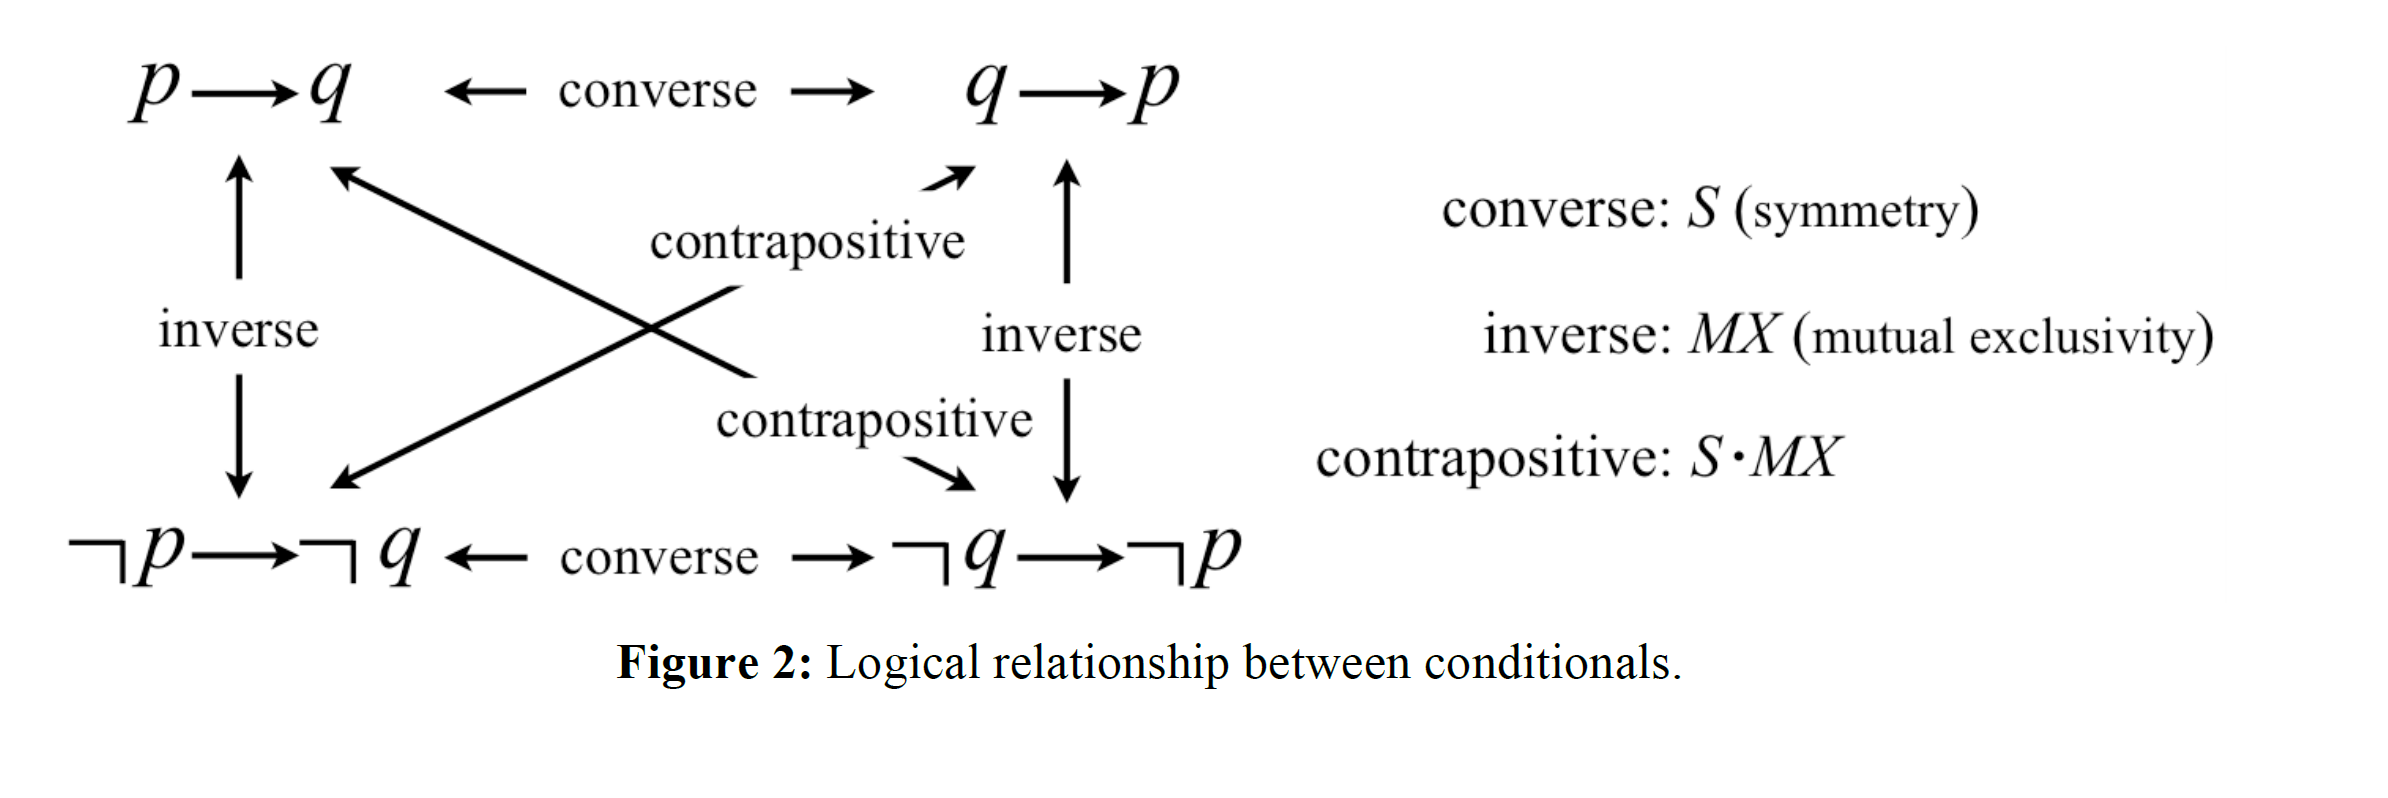
\includegraphics[width=0.98\textwidth]{images/cong23.png}
    \caption{Relation between cognitive biases.}
    \label{cong23}
\end{figure}

\noindent Note: From “Cognitive Symmetry: Illogical but Rational Biases” by T. Takahashi, M. Nakano, and S. Shinohara, Symmetry Culture and Science. 21. 1-3, p. 7 \url{https://www.researchgate.net/publication/285850238_Cognitive_Symmetry_Illogical_but_Rational_Biases}~\cite{cogn}.
\vspace{10pt}

It is not always easy to see that the connection is off in the example. However, if we take an example where $p$ is “the shoe is white” and q “a star is printed on it,” symmetric bias infers “if a star is printed on a shoe, then the shoe is white” ($q \implies p$) and mutual exclusivity bias infers “if the shoe is not white, then a star is not printed on it” ($\neg p \implies \neg q$) which are certainly not correct to assume from hearing “if the shoe is white, then a star is printed on it ($p \implies q$)”~\cite{els}.

The Table~\ref{co-occorj} shows the co-occurrence table of $p$ and $q$'s relationships.

\begin{table}[H]
    \centering
    \begin{tabular}{| c ||c| c|}
    \hline
         & $q$ & $\neg q$  \\
         \hline
         $p$& $a$ & $b$\\
         \hline
         $\neg p$ & $c$ & $d$\\
         \hline
    \end{tabular}
    \caption{Co-occurrence frequency for event $p$ and event $q$.}
    \label{co-occorj}
\end{table}

\noindent Note: Adapted from “Self‑incremental learning vector
quantization with human cognitive
biases” by N. Manome, S. Shinohara, T. Takahashi, Y. Chen, and U. Chung, Scientific Reports 11(1), p. 3 (\url{https://doi.org/10.1038/s41598-021-83182-4})~\cite{lrimp}.
\vspace{10pt}

We can map the logic relations to machine learning logic by assuming $p$ as \textit{the predicted label is prototype i’s label} and $q$ as \textit{the predicted result is correct}, provided by Manome (2021)~\cite{lrimp}. If we take $L(\mathbb{x})$ as the sample $\mathbb{x}$ label, $L(\omega^{\mathbb{x}})$ as the predicted prototype label (or winner class for short) of sample $\mathbb{x}$, and $L(\omega_{i}$) as prototype $i$’s label, then the co-occurrence frequency table be like in the Table~\ref{co-occ}.


\begin{table}[H]
\centering
\begin{tabular}{| c ||c| c| }
\hline
  & $L(\mathbb{x}) = L(\omega^{\mathbb{x}}) (q)$ & $L(\mathbb{x}) \neq L(\omega^{\mathbb{x}}) (\neg q)$\\[0.5ex]
 \hline\hline
 $L(\omega_{i}) = L(\omega^{\mathbb{x}}) (p)$ &$a_{i}$ &$b_{i}$ \\
 \hline
 $L(\omega_{i}) \neq L(\omega^{\mathbb{x}}) (\neg p)$ & $c_{i}$ & $d_{i}$ \\
 \hline
\end{tabular}
\caption{Co-occurrence frequency for each prototype $\omega_{i}$.}
\label{co-occ}
\end{table}

\noindent Note: Adapted from “Self‑incremental learning vector
quantization with human cognitive
biases” by N. Manome, S. Shinohara, T. Takahashi, Y. Chen, and U. Chung, Scientific Reports 11(1), p. 5 (\url{https://doi.org/10.1038/s41598-021-83182-4})~\cite{lrimp}.
\vspace{10pt}

We defined two biases (S and MX), and now we define other essential properties of the probabilistic model. One is excluded middle (XM), a natural condition of whether an event occurs, and another one is called estimation relativity (ER)~\cite{cogn}. Below in Table~\ref{biastable}, we list the biases and properties respective to their logical dictation~\cite{cogn}. $B$ denotes the probabilistic formula, and $B(q|p)$ represents how strong someone subjectively believes that $q$ occurs after $p$ happened~\cite{cogn}. If the relationship holds, we say $B$ has the respective bias or property.

\begin{table}[H]
\centering
\begin{tabular}{c c}
Symmetry bias (S): &$B(q|p) \sim B(p|q)$\\[0.5ex]
\\
Mutual exclusivity bias (MX): &$B(q|p) \sim B(\neg q|\neg p)$\\[0.5ex]
\\
The law of excluded middle (XM): &$B(q|p) \sim 1- B(\neg q | p)$\\[0.5ex]
\\
Estimation relativity (ER): &$B(q|p) \sim 1- B(q|\neg p)$\\[0.5ex]
\end{tabular}
\caption{Biases, bias properties.}\label{biastable}
\end{table}

\noindent Note: Adapted from “Cognitive Symmetry: Illogical but Rational Biases” by T. Takahashi, M. Nakano, and S. Shinohara, Symmetry Culture and Science. 21. 1-3, p. 7 \url{https://www.researchgate.net/publication/285850238_Cognitive_Symmetry_Illogical_but_Rational_Biases}~\cite{cogn}.
\vspace{10pt}

There are many ways to implement one or a couple of these logical biases in learning rate optimizers. Since we do not want to clutter the paper with many cognitive learning rate optimizers, we filter and pick the ones that show higher performance according to Table~\ref{cogntable}.

\begin{table}[H]
\centering
\begin{tabular}{c c c c c c c c}
&\textbf{CP}&\textbf{DP}&\textbf{DFH}&\textbf{RS}&\textbf{MS$_{1,0}$}&\textbf{LS}&\textbf{LSR}\\
\hline\\
\textbf{H03}&0.000&0.000&0.964&0.158&0.968&0.969&0.971\\
\textbf{AS95}&0.823&0.781&0.905&0.761&0.885&0.904&0.782\\
\textbf{WDK90}&0.944&0.844&0.961&0.888&0.962&0.969&0.922\\
\end{tabular}
\caption{Determination coefficients of cognitive models.}
\label{cogntable}
\end{table}

\noindent Note: The text and human data collected from Hattori (2003) (H03)~\cite{hattori03}, Anderson \& Sheu (1995) (AS95)~\cite{ander95}, and Wasserman et al. (1990) (WDK90)~\cite{wasser}.
\vspace{5pt}

\noindent Note: Adapted from “Cognitive Symmetry: Illogical but Rational Biases” by T. Takahashi, M. Nakano, and S. Shinohara, Symmetry Culture and Science. 21. 1-3, p. 15 \url{https://www.researchgate.net/publication/285850238_Cognitive_Symmetry_Illogical_but_Rational_Biases}~\cite{cogn}.


\paragraph{CGLVQ optimizers}



\subparagraph{CP model}

This model is a conditional probability (CP) model. The model is the most basic among others. CP only satisfies XM~\cite{cogn}. If we use the probability notation $p,q$ and the Table~\ref{co-occ}, $t$ for time, the causal relationship between events ($R(t)$) of the CP would be the following~\cite{cogn,lrimp}:
\vspace{10pt}

\begin{equation}
R^{\text{CP}(q|p)}(t) = \frac{a(t)}{a(t)+b(t)}
\end{equation}
\vspace{10pt}

We can see that CP satisfies XM by looking at the following equation~\cite{cogn}:
\vspace{10pt}


\begin{equation}
\begin{split}
R^{\text{CP}(q|p)}(t) &= \frac{a(t)}{a(t)+b(t)}\\
\\
&= 1 - \frac{b(t)}{a(t)+b(t)}\\
\\
&= 1- R^{\text{CP}(\neg p|q)}(t)
\end{split}
\end{equation}


\subparagraph{DFH model}

The Dual factor heuristic (DFH) model (cited from Takahashi et al. (2010)~\cite{cogn} which cites from Hattori (2001)~\cite{hattori01} Japanese translation and Hattori (2003)~\cite{hattori03}) is one of the models that work best for a human-like model~\cite{hattori07,cogn}. DFH is derived from CP and defined by the product of CP and its inverse~\cite{cogn}:
\vspace{10pt}

\begin{equation}
\begin{split}
R^{\text{DFH}(q|p)}(t) &= \sqrt{ R^{\text{CP}(q|p)}(t) \cdot R^{\text{CP}(p|q)}(t)}\\
\\
&= \frac{a(t)}{\sqrt{[a(t)+b(t)]\cdot [a(t)+c(t)]}}
\end{split}
\end{equation}
\vspace{10pt}

 DFH satisfies the S bias, as we can see in the following equation~\cite{cogn}:
\vspace{10pt}

\begin{equation}
\begin{split}
R^{\text{DFH}(q|p)}(t) &= \sqrt{ R^{\text{CP}(q|p)}(t) \cdot R^{\text{CP}(p|q)}(t)}\\
\\
&= \sqrt{ R^{\text{CP}(p|q)}(t) \cdot R^{\text{CP}(q|p)}(t)}\\
\\
&= R^{\text{DFH}(p|q)}(t)
\end{split}
\end{equation}
\vspace{10pt}


\subparagraph{MS model}

According to Takahashi et al. (2010), ~\cite{cogn}, representing human cognition, we should use neither too much symmetry nor no symmetry but somewhere in between. That is why we have a middle symmetry (MS) model. MS has parameters $\alpha$ and $\beta$ to control the magnitude of the symmetry. MS$_{\alpha,\beta}$ has the following equation~\cite{cogn}:
\vspace{10pt}

\begin{equation}
R^{\text{MS}_{\alpha,\beta}(q|p)}(t) = \frac{a(t) + \beta\cdot d(t)}{a(t)+ \beta\cdot d(t) + b(t) + \alpha\cdot c(t)}
\end{equation}
\vspace{10pt}

MS$_{0,0}$ corresponds to the CP model. According to Takahashi et al. (2010)~\cite{cogn}, when $\alpha = 1$ and $\beta = 0$, Hattori (2003) achieved good performance with \textit{Human} dataset with causal inductive experiments~\cite{cogn,hattori03}. With the given parameters, MS$_{1,0}$ equation would look like~\cite{cogn}:
\vspace{10pt}

\begin{equation}
R^{\text{MS}_{1,0}(q|p)}(t) = \frac{a(t)}{a(t) + b(t) + c(t)}
\end{equation}
\vspace{10pt}

MS$_{1,0}$ is symmetric, so it has S bias but lacks MX bias~\cite{cogn}.

We use MS$_{1,0}$ model in this paper, and from now on, we mention MS$_{1,0}$ as MS for simplicity.

\subparagraph{LS model}

Loose symmetry derived from the CP model is used as a parameter in the MS model to create a model with both S and MX biases. For LS, we take $\alpha = R^{\text{CP}(p|q)}(t) = \frac{a(t)}{a(t)+c(t)}$ and $\beta = R^{\text{CP}(p|\neg q)}(t) = \frac{b(t)}{b(t)+d(t)}$ in $R^{\text{MS}_{\alpha,\beta}(q|p)}(t)$. According to Takahashi et al. (2010)~\cite{cogn}, which sources the Japanese translation of Shinohara et al. (2007)~\cite{shinohara}, reported performing well in purely inductive and decision-theoretic (recursively inductive-deductive) tasks. The equation of LS is~\cite{cogn,lrimp}:
\vspace{10pt}

\begin{equation}
R^{\text{LS}(q|p)}(t) = \frac{a(t) + \frac{b(t)}{b(t)+d(t)} d(t)}{a(t)+ \frac{b(t)}{b(t)+d(t)} d(t) + b(t) + \frac{a(t)}{a(t)+c(t)} c(t)}
\end{equation}
\vspace{10pt}

LS model satisfies XM and loosely satisfies S, MX biases, and ER~\cite{cogn}.


\subparagraph{LSR model}

The final model we use is loose symmetry under the rarity assumption (LSR)~\cite{cogn}. As we can understand from the name, LSR derives from the LS model. The rarity assumption~\cite{oaksford} has been considered important in human causal inference. The assumption here is, that events $p$ and $q$ probabilities are small, which makes $d(t) = P(\neg p| \neg q)$ much higher than other components since the correlation of any two events is highly unlikely~\cite{hattori07}. For example, any random event and you start your car in the morning are most likely not correlated with each other~\cite{hattori07}. The equation of LSR can be achieved by diverging $d(t) \rightarrow \infty$ in the LS model~\cite{cogn}.
\vspace{10pt}

\begin{equation}
\begin{split}
R^{\text{LSR}(q|p)}(t) &= lim_{d(t) \rightarrow \infty} R^{\text{LS}(q|p)}(t)\\
\\
&= lim_{d \rightarrow \infty} \frac{a(t) + \frac{b(t)}{b(t)+d(t)} d(t)}{a(t)+ \frac{b(t)}{b(t)+d(t)} d(t) + b(t) + \frac{a(t)}{a(t)+c(t)} c(t)}\\
\\
&= \frac{a(t)+b(t)}{a(t)+2b(t)+ \frac{a(t)}{a(t)+c(t)} c(t)}
\end{split}
\end{equation}
\vspace{10pt}

According to the Table~\ref{cogntable} from Takahashi et al. (2010)~\cite{cogn}, LSR fits the \textit{Human} data from \textit{H03}~\cite{hattori03} slightly better than LS.
\vspace{10pt}

\noindent The Python code of the optimizers can be found in \hyperlink{appoptim}{Appendix A} or on the following GitHub page:

\noindent \url{https://github.com/mertsaru/Cognitive-GLVQ/blob/main/optimizer.py}

\subsubsection{Updating learning rates with CGLVQ}

The learning rate update of any CGLVQ optimizer is described in Figure~\ref{flowchart}. The methods first count the co-occurrence frequency for all the prototypes in each training sample to calculate $R_{i}$ of each $\omega_{i}$. After finding the co-occurrence frequency of the given $\omega_{i}$, the $R_{i}$ is calculated by the chosen cognitive science learning rate optimizer method according to Manome et al. (2021)~\cite{lrimp}.

\begin{figure}[H]
    \centering
    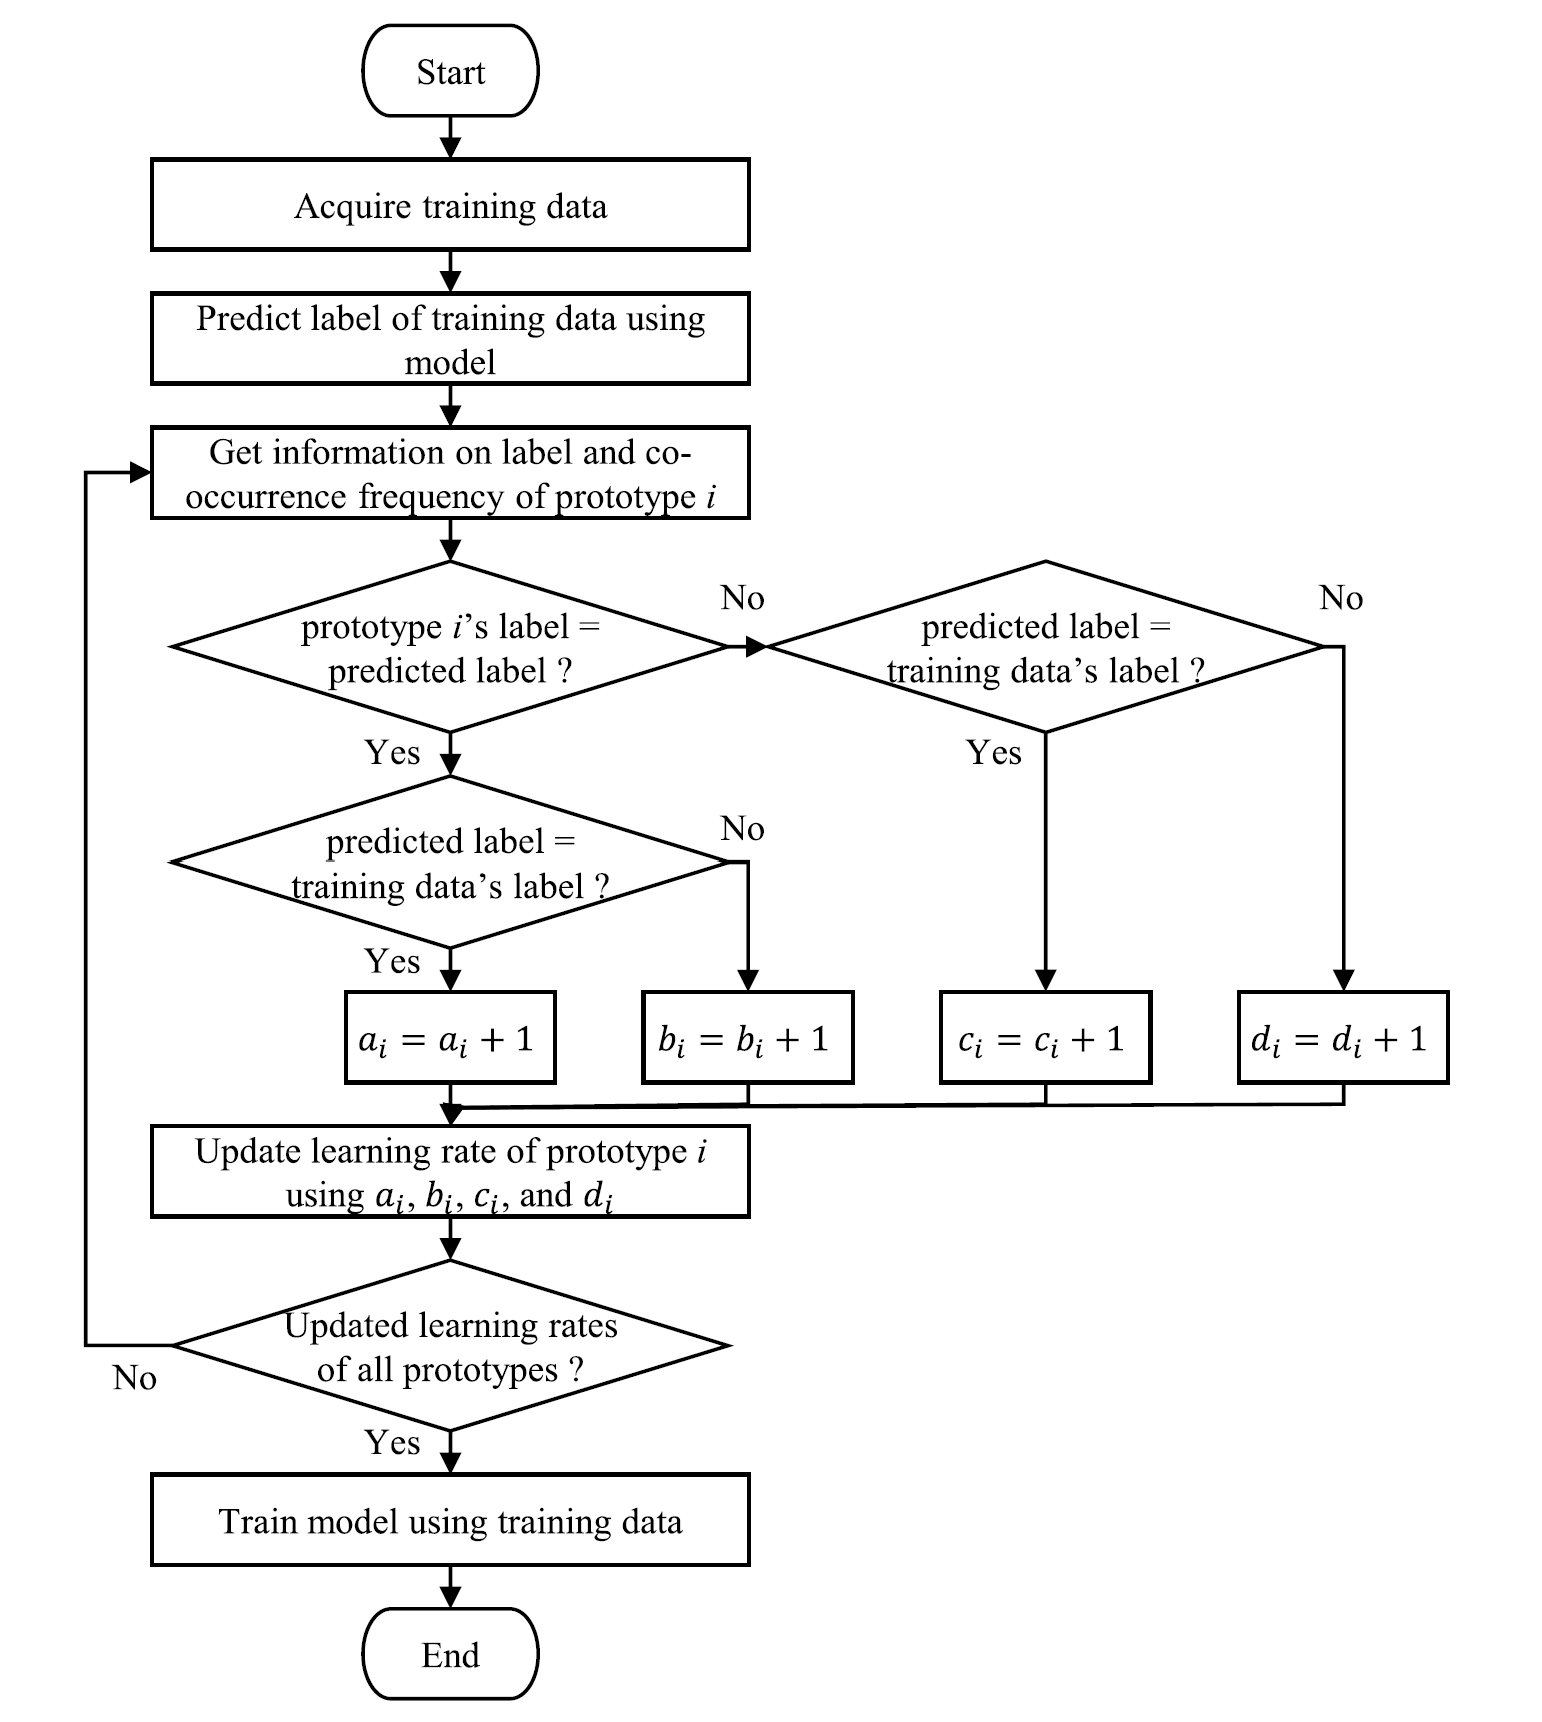
\includegraphics[width=0.98\textwidth]{images/lr flowchart.png}
    \caption{Training structure of CGLVQ models.}
    \label{flowchart}
\end{figure}

\noindent Note: From “Self‑incremental learning vector
quantization with human cognitive
biases” by N. Manome, S. Shinohara, T. Takahashi, Y. Chen, and U. Chung, Scientific Reports 11(1), p. 3 (\url{https://doi.org/10.1038/s41598-021-83182-4})~\cite{lrimp}.
\vspace{10pt}

After finding the $R_{i}(t)$ of the $\omega_{i}(t)$ we can calculate its $\epsilon_{i}(t)$ at time $t$ by~\cite{lrimp}:

\begin{equation}
\epsilon_{i}(t) = 1 - R_{i}(t)\label{alphar}
\end{equation}

However, the Equation~\eqref{alphar} would give us $\epsilon_{i}(t) \in [0,1]$, since $R_{i}(t) \in [0,1]$ for any CGLVQ learning rate optimizer and $\forall t \in [0,\infty)$. To adjust the $\epsilon_{i}(t)$ of the model to the range of $\epsilon_{i}(0)$, we take $\epsilon_{i}(t)$ as:

\begin{equation}
\epsilon_{i}(t) = \epsilon(0)(1 - R_{i}(t))
\end{equation}

to make $\epsilon_{i}(t)\in [0, \epsilon(0)], \forall t \in [0, \infty)$.
\vspace{10pt}

\noindent The Python code of CGLVQ can be found in \hyperlink{appcglvq}{Appendix A} or on the following GitHub page:

\noindent \url{https://github.com/mertsaru/Cognitive-GLVQ/blob/main/cognitive_GLVQ.py}


\section{Test Measures}

When training the data, we need a measure to understand how useful the machine learning classification model is. For that, we have different types of test measures. The most used and well-known method is the accuracy method, which is useful when the classes have an equal or close number of (balanced) samples in the dataset. If the sample numbers for classes are not equal (imbalanced), we have an F score to have a prediction power of the method. According to Kaden et al. (2014)~\cite{kaden}, the F score performs better for the dataset with imbalanced class samples than for accuracy.

Another way to deal with datasets that have imbalanced class samples is to create artificial data for the missing classes. These methods are either using Generative AI to create artificial data from scratch or using data augmentation methods on the existing data to stretch, discolor, rotate, and more on the existing data to create new samples. However, these artificial data creation methods are not always helpful. There are some datasets that one cannot create artificially. Secondly, using a Generative adversarial network (GAN) to generate new data would also have problems since we need labels for generated data. However, finding the labels in the original data is hard for the human eye, and we do not have a label-generating model for the unlabeled data. So, we do not discuss how to create data artificially, but we talk about what we can do when we have a dataset where the classes are imbalanced.


\subsubsection{Accuracy score}

Accuracy is easy to understand and apply. We predict everything in the test set after training the model with the training set. To get the accuracy score, we divide the correctly predicted samples by the number of all samples in the test set, like in Equation~\ref{acc}.
\vspace{10pt}

\begin{equation}
\text{accuracy score} = \frac{\text{\# correct classification}}{\text{\# total samples}}\label{acc}
\end{equation}
\vspace{10pt}

As we mentioned earlier, the accuracy is reasonable when the samples for each class are balanced. Let us examine what would happen if we use accuracy on an imbalanced sample of classes. For this example, we assume that the Test dataset 1 has 100 samples where 99 have class label 0 and 1 has class label 1. Let the model for classification label every input to class label 0. Then, according to the accuracy equation, the model’s accuracy would be $99\%$ for Test dataset 1~\eqref{acc1}. If we calculate the accuracy for the same model but with an evenly distributed test dataset, where Test dataset 2 has 50 samples for class 0 and 50 samples for class 1 out of 100, the accuracy would be $50\%$ with Test dataset 2~\eqref{acc2}. So, with an unequal number of samples for each class, accuracy would be a misinterpretation of the model’s prediction reliability.
\vspace{10pt}

\begin{subequations}
\renewcommand{\theequation}{\theparentequation.\arabic{equation}}
\noindent Test set 1 accuracy score:
    \begin{equation}
\frac{\text{\# correct classification}}{\text{\# total samples}} = \frac{99}{100} = 99\%\label{acc1}
    \end{equation}
Test set 2 accuracy score:
    \begin{equation}
\frac{\text{\# correct classification}}{\text{\# total samples}} = \frac{50}{100} = 50\%\label{acc2}
    \end{equation}
    \end{subequations}


\subsubsection{F score}

F1 score, or more generally F$_{\beta}$ score, comes in handy when we cannot rely on accuracy measurement. The F1 score is a subclass of F$_{\beta}$ score, which is calculated by recall ($\rho$) and precision ($\pi$) of the model. We need to dive into prediction cases to understand the recall and precision. We start with the binary classification model.

Let us start naming the classes as class 0 and class 1. For every prediction in a binary classification model, we have four options:

\begin{itemize}
    \item The model predicts the sample $\mathbb{x}$ belongs to class 0, and it is correct (True positive (TP))
    \item The model predicts the sample $\mathbb{x}$ belongs to class 0, and it is wrong (False positive (FP))
    \item The model predicts the sample $\mathbb{x}$ belongs to class 1, and it is correct (True negative (TN))
    \item The model predicts the sample $\mathbb{x}$ belongs to class 1 and it is wrong (False negative (FN))
\end{itemize}

If $L(\mathbb{x})$ represents the label of $\mathbb{x}$ and $L(\omega^{\mathbb{x}})$ represents the prediction label of $\mathbb{x}$, then we can see the confusion matrix of class 0 in Table~\ref{conf matrix}.

\begin{table}[H]
\centering
\begin{tabular}{| c ||c| c| }
\hline
  & $L(\mathbb{x}) = 0 $ & $L(\mathbb{x}) \neq 0$\\[0.5ex]
 \hline\hline
 $L(\omega^{\mathbb{x}}) = 0$ & TP & FP \\
 \hline
 $L(\omega^{\mathbb{x}}) \neq 0$ & FN  & TN \\
 \hline
\end{tabular}
\caption{Co-occurrence frequency for each prototype $\omega_{i}$.}
\label{conf matrix}
\end{table}

Then recall ($\rho$) and precision ($\pi$) follows as:
\vspace{10pt}

\begin{equation}
\rho = \frac{TP}{TP+FP}
\end{equation}
\begin{equation}
\pi = \frac{TP}{TP+FN}
\end{equation}
\vspace{10pt}

and the F$_{\beta}$-score for the model would be:
\vspace{10pt}

\begin{equation}
F_{beta} =  \frac{(1+\beta^{2})\cdot \pi \cdot \rho}{(\beta^{2}\cdot \pi) + \rho}
\end{equation}
\vspace{10pt}

Since we use the F1 score, the measurement we use in our results would be:
\vspace{10pt}

\begin{equation}
F_{1} = \frac{2\pi\cdot\rho}{\pi + \rho}\label{f1score}
\end{equation}
\vspace{10pt}


The problem with F scores is that the score’s output does not tell us how reliable the model is. We know with what percentage the model predicts the samples for the accuracy score, but the F scores do not give us such an answer. Most of the time, the F score of one class is not equal to the second class’s F1 score in classification problems. If we check the example Table~\ref{confmax0}, for class 0, the F1 score is equal to $0.8$. The Table~\ref{confmax0} can be rewritten for class 1 as Table~\ref{confmax1}. However, when we check the F1 score of class 1 for the same table, the score would be $0.\bar{6}$. So, it is hard to understand what the F1 score means. However, it gives us a nice comparison between models and reflects the accuracy change of the model while using imbalanced samples for classes in the dataset.

\begin{table}[H]
\centering
\begin{tabular}{| c ||c| c| }
  \multicolumn{3}{c}{Class 0}\\
 \hline
& $L(\mathbb{x}) = 0 $ & $L(\mathbb{x}) \neq 0$\\[0.5ex]
 \hline\hline
$L(\omega^{\mathbb{x}}) = 0$ & $50$ & $5$ \\
 \hline
 $L(\omega^{\mathbb{x}}) \neq 0$ & $20$  & $25$ \\
 \hline
\end{tabular}
\caption{Example: confusion matrix for class 0.}
\label{confmax0}
\end{table}

\begin{table}[H]
\centering
\begin{tabular}{| c ||c| c| }
  \multicolumn{3}{c}{Class 1}\\
 \hline
& $L(\mathbb{x}) = 1 $ & $L(\mathbb{x}) \neq 1$\\[0.5ex]
 \hline\hline
$L(\omega^{\mathbb{x}}) = 1$ & $25$ & $20$ \\
 \hline
 $L(\omega^{\mathbb{x}}) \neq 1$ & $5$  & $50$ \\
 \hline
\end{tabular}
\caption{Example: confusion matrix of the Table~\ref{confmax0}, rewritten for class 1.}
\label{confmax1}
\end{table}

Regarding the Table~\ref{confmax0} and Table~\ref{confmax1} and using the F1 score on same $\omega^{\mathbb{x}}$, we achieve the following equations for each class:
\vspace{10pt}

\begin{equation}
F_{1}(\text{class = 0}) = \frac{2\cdot\frac{50}{55}\cdot\frac{50}{70}}{\frac{50}{55}+\frac{50}{70}}= 0.8
\end{equation}
\vspace{5pt}

\begin{equation}
F_{1}(\text{class = 1}) = \frac{2\cdot\frac{25}{45}\cdot\frac{25}{30}}{\frac{25}{45}+\frac{25}{30}}= 0.\bar{6}
\end{equation}
\vspace{10pt}

To get a single score for the dataset, we combine the F1 scores. F1 scores can be combined by taking the average of the scores or the average by multiplying each class’s weight with their corresponding F1 score, or we can examine the F1 scores for each class in a dataset separately. The latter would be hard to comprehend, and the average of all F1 scores has its own problems. In our analysis, we take the F1 score for each model epoch as the weighted average of the class F1 score. This method can be used to find common F1 scores for multiclassification problems.

So, to use accuracy as an effective measure, we conduct separate experiments. We select an equal number of samples for classes in the dataset to get accurate accuracy scores. Besides that, we also use the dataset with imbalanced class samples and examine the F1 score. By conducting two experiments with different sample sizes, we would investigate the models we use in different situations and better understand the models’ powers.

\section{The Experiments}

We used two experiments on the datasets in this paper. For both of the experiments, each dataset uses the same prototype set. First, we took an equal number of samples for each class in every dataset. In this experiment, the accuracy score is essential to look at. For our second test, we distributed the samples unevenly between classes. The second experiment compares F1 scores. We used two experiments with different sample sizes because, in real-world data, we do not have equally divided sample sizes most of the time. Sometimes, with unbalanced sample sizes, we can get different results than balanced sample sizes, and we want to see the models’ performance in both cases.

We ran the same experiment three times with different $\epsilon(0)$: $0.1$, $0.03$, and $0.01$. We randomly selected the prototypes and sample sets for each dataset in every experiment. After selecting the samples for the test set, training set, and prototypes, we used the same samples for each test and dataset. The prototypes are selected by comparing accuracy scores on experiment 1 using OGLVQ with $\epsilon(0)= 0.1$ and taking the prototype sample with the highest accuracy score among 20 different random $\omega$ set and dataset sampling. Prototype and dataset selection is still (semi-)random since we use seeds in random selection.

We have two plot graphs in both experiments for each test: the corresponding measure score of the experiment and learning rate values. We look at the learning rate values to see if the model is learning appropriately or not. Since $\epsilon_{i}$ differs for each prototype in GLVQ models, we have many learning rate plots in our graphs, differentiated labels by color. We associate learning rate in CGLVQ models with learning since learning rate in CGLVQ is positively related to $a$ ($L(\omega_{i}) = L(\omega^{\mathbb{x}}) \implies L(\mathbb{x}) = L(\omega^{\mathbb{x}}) $) in the Table~\ref{co-occ} in all the models, and $a$ is correctly predicted. So, an increase of $a$ would decrease the $\epsilon_{i}(t)$ since $\epsilon_{i}(t) = \epsilon(0) \cdot (1-R)$, and $R$ in positive relation with $a$ for all cognitive science learning rate optimizers.
